% Beamer slide deck for Mathematical Physics
% "Mathematical Physics"
% Chapter 6: Orthogonal Polynomials
% Self-contained slide text; local figures live in figs.

\documentclass[11pt]{beamer}

\usepackage[utf8]{inputenc}
\usepackage[T1]{fontenc}
\usepackage{lmodern}
\usepackage{amsmath,amssymb}
\usepackage{graphicx}

\usetheme{Madrid}

\author[]{Compiled by Jake W. Liu}
\title[Orthogonal Polynomials]{Chapter 6: Orthogonal Polynomials}
\subtitle{Mathematical Physics}
\date{\today}

\setbeamertemplate{navigation symbols}{}
\setbeamertemplate{frametitle continuation}[from second]

\AtBeginSection[]
{
 \begin{frame}<beamer>
 \frametitle{Table of contents}
 \tableofcontents[currentsection]
 \end{frame}
}

\usepackage{Kyushu}

% Neutralize \index so source markup (if any) is harmless.
\makeatletter
\@ifundefined{index}{\newcommand{\index}[1]{}}{\renewcommand{\index}[1]{}}
\makeatother

\begin{document}

\newcounter{sfchapter}
\setcounter{sfchapter}{6}
\renewcommand{\thesection}{\arabic{sfchapter}.\arabic{section}}
\numberwithin{equation}{section}

\begin{frame}[c]\titlepage
\end{frame}

\begin{frame}{Outline}
\tableofcontents
\end{frame}

\begin{frame}{Where we are going}
\footnotesize
This chapter studies four families of \textbf{orthogonal polynomials} that arise by
separating variables in Laplace, Poisson, Helmholtz, and Schr\"odinger problems.
``Orthogonal'' means a weighted inner product of distinct-degree polynomials vanishes;
the interval and weight depend on the family.

\smallskip
\textbf{The picture to keep in mind:} each family is a ``Fourier series'' basis for its own
interval and weight. To expand a function $f=\sum c_n\phi_n$, orthogonality reads off each
coefficient with one integral, $c_n=\int f\phi_n w\,dx\big/\!\int\phi_n^2w\,dx$, exactly as
for sines in Chapter~4.
\begin{itemize}
  \item \textbf{Legendre $P_n$.} From Laplace in spherical coordinates to the Legendre
        equation, generating function, recurrence, Rodrigues, orthogonality, and
        Fourier--Legendre expansions; then associated Legendre functions and spherical
        harmonics $Y_n^m$.
  \item \textbf{Hermite $H_n$.} The Hermite equation and series solution, quantum harmonic
        oscillator motivation, generating function, Rodrigues formula, and weighted
        orthogonality.
  \item \textbf{Laguerre $L_n$ and Chebyshev $T_n$.} Defining ODEs, first polynomials,
        weights and orthogonality, recurrences, and useful formula sheets.
\end{itemize}
A comparison table at the end collects interval, weight, and ODE for each family.
\end{frame}

% ======================================================================
\section{From Laplace to ordinary Legendre}
\label{sec:laplace-to-legendre}
% ======================================================================

\begin{frame}[allowframebreaks=1.00]{Two-dimensional Laplace equation in polar coordinates}
\footnotesize

\textbf{Why start in 2D.} Two conditions will pick the solutions here: a condition on the
angle fixes the separation constant, and regularity at the center keeps $r^n$. In 3D the same
two moves return (finiteness at the poles replaces periodicity) and produce Legendre polynomials.

\textbf{Step 1: separate the angular and radial parts.}  A function satisfying Laplace's equation $\nabla^2\psi=0$ (e.g.\ a steady temperature or an electrostatic potential in a charge-free region) is called a \emph{harmonic
function}. The operator $\nabla^2$ is the Laplacian: $\psi_{xx}+\psi_{yy}$ in
Cartesian coordinates. In polar coordinates $r$ is radius and $\theta$ is angle.
We use its coordinate form without deriving it:
\begin{equation}
  \nabla^2\psi
   = \frac{1}{r}\,\frac{\partial}{\partial r}\left(r\,\frac{\partial\psi}{\partial r}\right)
   + \frac{1}{r^2}\,\frac{\partial^2\psi}{\partial\theta^2} = 0.
  \label{eq:laplace2d}
\end{equation}
Take a separated solution $\psi(r,\theta)=u(r)v(\theta)$. Then $\psi_r=u'v$ and
$\psi_{\theta\theta}=uv''$, so \eqref{eq:laplace2d} becomes
\[
  \frac{v}{r}\left(ru'\right)'+\frac{u}{r^2}v''=0
  \quad\xrightarrow{\ \times r^2/(uv)\ }\quad
  \frac{r(ru')'}{u}+\frac{v''}{v}=0,
\]
and therefore
\begin{equation}
  -\frac{v''}{v}=\frac{r(ru')'}{u}=\lambda,
  \label{eq:laplace2d-separation}
\end{equation}
because the left member depends only on $\theta$ and the right member only on $r$.

\par\framebreak\par
\textbf{Step 2: the angular equation \(v''+\lambda v=0\).} Going once around the circle brings us back to
the same point, so \(v\) must be \(2\pi\)-periodic: \(v(\theta+2\pi)=v(\theta)\). Check each sign of \(\lambda\):
\begin{itemize}
  \item \(\lambda>0\), write \(\lambda=\mu^2\): \(v=A\cos\mu\theta+B\sin\mu\theta\). This has period \(2\pi\) only if \(\mu\) is a
        whole number \(n\). So \(\lambda=n^2\), \(n=1,2,\dots\).
  \item \(\lambda=0\): \(v=A+B\theta\). Periodic only if \(B=0\): the constant mode, which we call \(n=0\).
  \item \(\lambda<0\): \(v\) is a combination of \(e^{\pm\sqrt{-\lambda}\,\theta}\), never periodic. Not allowed.
\end{itemize}
So \(\lambda=n^2\) with \(n=0,1,2,\ldots\). \emph{The periodicity condition forced the integer \(n\).}

\textbf{Step 3: the radial equation.} With \(\lambda=n^2\), \eqref{eq:laplace2d-separation} gives \(r(ru')'=n^2u\).
Expand \((ru')'=ru''+u'\):
\begin{equation}
  r^2u''+ru'-n^2u=0.
  \label{eq:laplace2d-radial}
\end{equation}
This is a Cauchy--Euler equation, so try \(u=r^p\): \(r^2p(p-1)r^{p-2}+r\,pr^{p-1}-n^2r^p=(p^2-n^2)r^p=0\).
So \(p=\pm n\) for \(n\ge1\): \(u=r^n\) or \(r^{-n}\). For \(n=0\) the equation is \((ru')'=0\), so \(ru'=C_0\),
\(u'=C_0/r\), and \(u=D_0+C_0\log r\).

\textbf{Step 4: regularity at the center.} On an annulus (\(r\) away from \(0\)), all these radial solutions are
allowed. But inside a disk that contains \(r=0\), the solution must stay finite there, and \(\log r\) and
\(r^{-n}\) blow up. Keeping only \(r^n\):
\begin{equation}
  \psi(r,\theta)
   =A_0+\sum_{n=1}^{\infty}r^n
       \bigl[A_n\cos(n\theta)+C_n\sin(n\theta)\bigr].
  \label{eq:laplace2d-sol}
\end{equation}
The lesson carried to 3D: the \emph{angular condition} (here periodicity) forced the
integer $n$, and \emph{regularity at the center} kept only $r^n$.
\end{frame}

\begin{frame}[allowframebreaks=1.00]{Three-dimensional Laplace equation in spherical coordinates}
\footnotesize

\textbf{Goal.} Solve Laplace's equation $\nabla^2\psi=0$ outside or inside a sphere, for example
the potential of charges near a sphere. Separation of variables will split it into a radial
equation, solved here, and an angular equation, solved on the next frames, whose solutions are
the Legendre polynomials.

In spherical coordinates $r$ is radius, $\theta$ is the polar angle measured from
the positive vertical axis, and $\phi$ is the azimuthal angle around that axis.
We use the spherical Laplacian without deriving this coordinate formula:
\begin{equation}
  \nabla^2\psi
  =
  \frac{1}{r^2}
    \frac{\partial}{\partial r}
      \left(r^2\frac{\partial\psi}{\partial r}\right)
  +\frac{1}{r^2\sin\theta}
    \frac{\partial}{\partial\theta}
      \left(\sin\theta\frac{\partial\psi}{\partial\theta}\right)
  +\frac{1}{r^2\sin^2\theta}
    \frac{\partial^2\psi}{\partial\phi^2}
  =0.
  \label{eq:laplace3d}
\end{equation}

\textbf{Step 1: separate the radial variable.}  Set $\psi(r,\theta,\phi)=u(r)y(\theta,\phi)$.
Because $y$ is independent of $r$ and $u$ is independent of the angles,
$\partial_r(r^2\psi_r)=y(r^2u')'$ and $\partial_\theta(\sin\theta\,\psi_\theta)=u(\sin\theta\,y_\theta)_\theta$.
Substitution into \eqref{eq:laplace3d} and multiplication by $r^2/(uy)$ give
\begin{equation}
  \frac{(r^2u')'}{u}
  =
  -\frac{
      \dfrac{1}{\sin\theta}(\sin\theta\,y_\theta)_\theta
      +\dfrac{1}{\sin^2\theta}y_{\phi\phi}
    }{y}
  =\lambda.
  \label{eq:sep-radial3d}
\end{equation}
The first expression depends only on $r$ and the second only on
$(\theta,\phi)$, so each equals a constant $\lambda$.

\par\framebreak\par
\textbf{Step 2: radial Euler equation.}  Expanding $(r^2u')'=r^2u''+2ru'$ gives
$r^2u''+2ru'-\lambda u=0$. Try $u=r^\sigma$: since $u'=\sigma r^{\sigma-1}$ and
$u''=\sigma(\sigma-1)r^{\sigma-2}$, we get
$r^2u''+2ru'=[\sigma(\sigma-1)+2\sigma]r^\sigma=\sigma(\sigma+1)r^\sigma$, so
$[\sigma(\sigma+1)-\lambda]r^\sigma=0$ and $\lambda=\sigma(\sigma+1)$.  Once the angular problem forces
$\lambda=n(n+1)$ with $n=0,1,2,\ldots$ (next frames), the exponent equation
$\sigma(\sigma+1)=n(n+1)$ factors as
\[
  \sigma^2+\sigma-n(n+1)=(\sigma-n)(\sigma+n+1)=0
  \quad\Longrightarrow\quad
  \sigma=n,\qquad \sigma=-n-1,
\]
and
\begin{equation}
  u_n(r)=A_nr^n+B_nr^{-n-1}.
  \label{eq:spherical-radial-powers}
\end{equation}
The $r^n$ branch is regular at the origin; the $r^{-n-1}$ branch decays at infinity.

The remaining angular eigenproblem is
\[
  \frac{1}{\sin\theta}
    \frac{\partial}{\partial\theta}
      \left(\sin\theta\,\frac{\partial y}{\partial\theta}\right)
  +\frac{1}{\sin^2\theta}\frac{\partial^2y}{\partial\phi^2}
  +\lambda y=0.
\]
We first treat the \textbf{axisymmetric} case (no $\phi$-dependence), which yields the
ordinary Legendre equation and $\lambda=n(n+1)$.  Associated Legendre modes for
$m\neq0$ come later as a short extension.
\end{frame}

\begin{frame}[allowframebreaks=1.00]{Axisymmetry: the ordinary Legendre equation}
\footnotesize

\textbf{Goal.} Solve the angular equation from the previous frame in the axisymmetric case, and
find which values of the separation constant $\lambda$ give a solution that is finite at both
poles. The answer is $\lambda=n(n+1)$, with the Legendre polynomials $P_n$ as the solutions.

\textbf{Step 1: assume no azimuthal dependence and change variables.}  If $\psi$ is independent of $\phi$
(axisymmetry about the polar axis), the angular eigenproblem at the end of the previous frame, with $y=v(\theta)$, reduces to
\[
  \frac{1}{\sin\theta}
    \frac{d}{d\theta}
      \left(\sin\theta\,\frac{dv}{d\theta}\right)
  +\lambda v=0.
\]
Set $x=\cos\theta$, so $dx/d\theta=-\sin\theta$ and $d/d\theta=-\sin\theta\,d/dx$.
Then
\begin{align*}
  \sin\theta\,\frac{dv}{d\theta}
    &=\sin\theta\,(-\sin\theta\,v_x)=-\sin^2\theta\,v_x=-(1-x^2)v_x,\\
  \frac{d}{d\theta}\left(\sin\theta\,\frac{dv}{d\theta}\right)
    &=-\sin\theta\frac{d}{dx}\bigl[-(1-x^2)v_x\bigr]
     =\sin\theta\frac{d}{dx}\bigl[(1-x^2)v_x\bigr],
\end{align*}
using $\sin^2\theta=1-\cos^2\theta=1-x^2$. Dividing the second line by $\sin\theta$ and
inserting it into the angular equation, we obtain
\begin{equation}
  \frac{d}{dx}\left[(1-x^2)v'(x)\right]+\lambda v(x)=0.
  \label{eq:legendre-eq-lambda}
\end{equation}
Expanding the derivative gives the equivalent form
\begin{equation}
  (1-x^2)v''-2xv'+\lambda v=0.
  \label{eq:legendre-eq-expanded-lambda}
\end{equation}

\textbf{Step 2: power series and coefficient recurrence.}  Set $v(x)=\sum_{j\ge0}a_jx^j$.
Writing every term as a series in $x^j$,
\begin{align*}
  v''
   &=\sum_{j\ge0}(j+2)(j+1)a_{j+2}x^j,\\
  -x^2v''
   &=-x^2\sum_{j\ge2}j(j-1)a_jx^{j-2}
    =-\sum_{j\ge0}j(j-1)a_jx^j,\\
  -2xv'
   &=-2x\sum_{j\ge1}j\,a_jx^{j-1}
    =-2\sum_{j\ge0}j\,a_jx^j.
\end{align*}
(Starting the last two sums at $j=0$ adds only terms with a factor $j(j-1)$ or $j$, which vanish.)
Substitution into \eqref{eq:legendre-eq-expanded-lambda}, with $-j(j-1)-2j=-j(j+1)$, gives
\[
  0=\sum_{j\ge0}
    \left[
      (j+2)(j+1)a_{j+2}
      +\bigl(\lambda-j(j+1)\bigr)a_j
    \right]x^j,
\]
so every coefficient vanishes and
\begin{equation}
  a_{j+2}
   =-\frac{\lambda-j(j+1)}{(j+2)(j+1)}\,a_j.
  \label{eq:legendre-coeff-recurrence-lambda}
\end{equation}
Even and odd chains are independent.

\textbf{Step 3: select solutions that remain finite at the poles.}
The points $x=\pm1$ are the north and south poles of the sphere, and a polynomial is
finite at both. The recurrence \eqref{eq:legendre-coeff-recurrence-lambda} stops exactly
when its numerator $\lambda-j(j+1)$ vanishes at some $j=n$, i.e.\ when $\lambda=n(n+1)$.
Then the numerator factors,
$n(n+1)-j(j+1)=(n^2-j^2)+(n-j)=(n-j)(n+j+1)$, and
\begin{equation}
  a_{j+2}
   =-\frac{(n-j)(n+j+1)}{(j+2)(j+1)}\,a_j.
  \label{eq:legendre-coeff-recurrence}
\end{equation}
At $j=n$ one has $a_{n+2}=0$, so the chain of the same parity as $n$ is a polynomial of
degree $n$. We quote the standard endpoint result: for any other $\lambda$ no nonzero
solution is finite at both poles, and for $\lambda=n(n+1)$ the other chain diverges at a pole,
so the finite solutions are the multiples of this polynomial.

\emph{Why the other chain must be discarded.} Take $\lambda=2=1\cdot2$ ($n=1$). The odd
chain stops at once and gives $v=x$. The \emph{even} chain with $a_0=1$ gives
\[
  a_2=-\frac{2-0}{2\cdot1}=-1,\qquad
  a_4=-\frac{2-6}{4\cdot3}(-1)=-\frac13,\qquad
  a_6=-\frac{2-20}{6\cdot5}\left(-\frac13\right)=-\frac15,
\]
and in general \(a_{2k}=-1/(2k-1)\). (Check: by \eqref{eq:legendre-coeff-recurrence-lambda} with \(\lambda=2\), \(j=2k\), the
ratio is \(a_{2k+2}/a_{2k}=[2k(2k+1)-2]/[(2k+2)(2k+1)]\). The numerator factors as
\(4k^2+2k-2=2(2k-1)(k+1)\) and the denominator as \(2(k+1)(2k+1)\), so the ratio is
\(\frac{2k-1}{2k+1}\), which is exactly the ratio of \(-\frac1{2k+1}\) to \(-\frac1{2k-1}\).) So
\[
  v(x)=1-x^2-\frac{x^4}{3}-\frac{x^6}{5}-\cdots=1-x\Bigl(x+\frac{x^3}{3}+\frac{x^5}{5}+\cdots\Bigr).
\]
The bracket is a known series: from \(\log(1\pm x)=\pm x-\frac{x^2}2\pm\frac{x^3}{3}-\cdots\), subtracting gives
\(\log(1+x)-\log(1-x)=2\bigl(x+\frac{x^3}{3}+\frac{x^5}{5}+\cdots\bigr)\). Hence
\[
  v(x)=1-\frac{x}{2}\log\frac{1+x}{1-x}.
\]
It is finite inside \((-1,1)\), yet \(v(x)\to-\infty\) as \(x\to1^-\) (because \(\log\frac{1+x}{1-x}\to\infty\)): it blows
up at the north pole, so it is useless on the sphere.
As quoted, the same happens for every $n$, so we set the starting coefficient of the
opposite-parity chain to zero.

With $\lambda=n(n+1)$, equations \eqref{eq:legendre-eq-lambda}--\eqref{eq:legendre-eq-expanded-lambda}
become the ordinary Legendre equation
\begin{equation}
  \frac{d}{dx}\left[(1-x^2)v'\right]+n(n+1)v=0,
  \quad\text{i.e.}\quad
  (1-x^2)v''-2xv'+n(n+1)v=0.
  \label{eq:legendre-eq}
\end{equation}
Choose the scale so that $P_n(1)=1$; the resulting polynomial is the
\emph{Legendre polynomial} $P_n$. Its powers are $x^n,x^{n-2},\ldots$ (the recurrence
advances by two), so $P_n(-x)=(-1)^nP_n(x)$.
The generating function (next section) produces all the $P_n$ with this normalization.
\end{frame}

% ======================================================================
\section{Legendre polynomials}
% ======================================================================

\begin{frame}[allowframebreaks=1.00]{Generating function from the Coulomb potential}
\footnotesize

We want all $P_n$ at once, with the normalization $P_n(1)=1$ built in. A point charge
supplies them. The goal is to show that
\[
 \frac1{\sqrt{1-2xt+t^2}}=\sum_{n=0}^{\infty}P_n(x)\,t^n,
\]
which is \eqref{eq:legendre-gen} below.

\textbf{Step 1: write the axisymmetric potential.}  Place a point charge one unit from the origin on the positive polar axis. For a field point
with spherical coordinates $(r,\theta,\phi)$, the law of cosines gives the distance to the charge,
$R^2=r^2+1^2-2r(1)\cos\theta=1-2r\cos\theta+r^2$, so, for a nonzero physical scale factor $C$, the Coulomb potential is
\begin{equation}
  \varphi(r,\theta)=\frac{C}{R}
  =\frac{C}{\sqrt{1-2r\cos\theta+r^2}}.
  \label{eq:coulomb}
\end{equation}
\begin{center}
  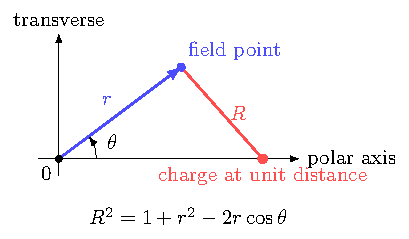
\includegraphics[width=0.42\linewidth]{figs/legendre_coulomb_geometry.pdf}
\end{center}
(The horizontal polar axis is a direction in space, not the variable $x=\cos\theta$.)

In the region $r<1$, which does not contain the charge, the potential is harmonic (as any
electrostatic potential away from charges), finite at the origin, and independent of $\phi$.
The separated solutions with these properties, $r^nP_n(\cos\theta)$ (the $r^n$ branch of
\eqref{eq:spherical-radial-powers} times $P_n$), suggest the expansion
\begin{equation}
  \frac{1}{\sqrt{1-2r\cos\theta+r^2}}
  =\sum_{n=0}^{\infty}a_n r^nP_n(\cos\theta).
  \label{eq:coulomb-expand}
\end{equation}

\textbf{Step 2: determine the coefficients on the axis.}  Set $\theta=0$. Then $\cos\theta=1$, $P_n(1)=1$ (the normalization chosen at the end of \S\ref{sec:laplace-to-legendre}), and
$1-2r\cos0+r^2=(1-r)^2$. Because $0\le r<1$, $|1-r|=1-r$, so \eqref{eq:coulomb-expand} becomes
$\sum_n a_nr^n=1/(1-r)=\sum_n r^n$ (geometric series). Uniqueness of power-series coefficients gives $a_n=1$.  Writing $t=r$ and $x=\cos\theta$,
\begin{equation}
  g(x,t)=\frac{1}{\sqrt{1-2xt+t^2}}
  =\sum_{n=0}^{\infty}P_n(x)t^n,
  \qquad |t|<1,\quad -1\le x\le1.
  \label{eq:legendre-gen}
\end{equation}
\par\framebreak\par
\textbf{Physical meaning.} For a far point ($r>1$), $1/R=r^{-1}g(\cos\theta,1/r)=\sum_n P_n(\cos\theta)/r^{n+1}$:
the \emph{multipole expansion} ($n=0$ monopole $1/r$, $n=1$ dipole $\cos\theta/r^2$);
$P_n$ is the angular pattern of the $n$-th multipole.

\textbf{Step 3: expand the first three $P_n$ from the generating function.}  Write
$g=(1-u)^{-1/2}$ with $u=2xt-t^2$ and use its Taylor series at $u=0$ (Chapter~1),
\[
  (1-u)^{-1/2}
    =1+\tfrac12 u+\tfrac12\cdot\tfrac32\frac{u^2}{2!}+O(u^3)
    =1+\tfrac12 u+\tfrac38 u^2+O(u^3).
\]
Since $u^2=(2xt-t^2)^2=4x^2t^2+O(t^3)$, collecting powers of $t$ up to $t^2$ gives
\begin{align*}
  g
    &=1+\tfrac12(2xt-t^2)+\tfrac38(4x^2t^2)+O(t^3)\\
    &=1+xt+\Bigl(-\tfrac12+\tfrac32 x^2\Bigr)t^2+O(t^3)\\
    &=1+xt+\tfrac12(3x^2-1)\,t^2+O(t^3).
\end{align*}
Matching powers of $t$ in $\sum P_n(x)t^n$ gives (each with $P_n(1)=1$, parity $(-1)^n$)
\begin{equation}
  P_0(x)=1,\qquad
  P_1(x)=x,\qquad
  P_2(x)=\frac12(3x^2-1).
  \label{eq:legendre-first-three}
\end{equation}
These agree with \S\ref{sec:laplace-to-legendre}: for $n=2$, \eqref{eq:legendre-coeff-recurrence}
gives $a_2=-3a_0$, i.e.\ $P_2\propto3x^2-1$.
\end{frame}

\begin{frame}[allowframebreaks=1.00]{Three-term recurrence}
\footnotesize

We want $P_{n+1}$ from the two previous polynomials, without another series expansion. The
goal is the relation
\[
 (n+1)P_{n+1}(x)=(2n+1)\,x\,P_n(x)-n\,P_{n-1}(x),
\]
which is \eqref{eq:legendre-recur} below; we get it from the generating function.

\textbf{Step 1: differentiate the generating function.}  Let
$D(x,t)=1-2xt+t^2$, so $g=D^{-1/2}$. Differentiating with respect to $t$ gives
\begin{align*}
  \frac{\partial g}{\partial t}
  &=-\frac12D^{-3/2}\frac{\partial D}{\partial t}
  =-\frac12D^{-3/2}(-2x+2t)
  =\frac{x-t}{D^{3/2}}.
\end{align*}
Termwise differentiation of the power series \eqref{eq:legendre-gen} gives
\begin{equation}
  \frac{\partial g}{\partial t}
  =\sum_{n=1}^{\infty}nP_n(x)t^{n-1}.
  \label{eq:dgdt}
\end{equation}
Multiplying $g_t=(x-t)D^{-3/2}$ by $D$ and using $D^{-1/2}=g$ gives $(x-t)g=Dg_t$.  Substituting both series \eqref{eq:legendre-gen} and \eqref{eq:dgdt},
\[
  (x-t)\sum_{n=0}^{\infty}P_nt^n
  =(1-2xt+t^2)\sum_{n=1}^{\infty}nP_nt^{n-1},
\]
where $P_n=P_n(x)$. Expanding,
\begin{align}
  \sum_{n=0}^{\infty}xP_nt^n
  -\sum_{n=0}^{\infty}P_nt^{n+1}
  &=\sum_{n=1}^{\infty}nP_nt^{n-1}
    -2\sum_{n=1}^{\infty}nxP_nt^n
    +\sum_{n=1}^{\infty}nP_nt^{n+1}.
  \label{eq:distribute}
\end{align}

\textbf{Step 2: compare coefficients of $t^n$.}  In \eqref{eq:distribute}, with the convention $P_{-1}=0$, the left coefficient of $t^n$ is $xP_n-P_{n-1}$.
On the right, writing $[t^n]$ for ``coefficient of $t^n$'',
\begin{gather*}
  [t^n]\sum_{j\ge1}jP_jt^{j-1}=(n+1)P_{n+1},
  \qquad
  [t^n]\bigl(-2\sum_{j\ge1}jxP_jt^j\bigr)=-2nxP_n,\\
  [t^n]\sum_{j\ge1}jP_jt^{j+1}=(n-1)P_{n-1}.
\end{gather*}
Equating coefficients,
\[
  xP_n-P_{n-1}
  =(n+1)P_{n+1}-2nxP_n+(n-1)P_{n-1}.
\]
Moving $-2nxP_n$ and $(n-1)P_{n-1}$ to the left,
$(1+2n)xP_n-(1+n-1)P_{n-1}=(n+1)P_{n+1}$, that is
\begin{equation}
  (n+1)P_{n+1}(x)
  =(2n+1)xP_n(x)-nP_{n-1}(x),
  \qquad n\ge0,
  \label{eq:legendre-recur}
\end{equation}
with $P_{-1}=0$ and $P_0=1$. For $n=0$, $P_1=xP_0=x$.
\end{frame}

\begin{frame}{First few Legendre polynomials}
\footnotesize
We already obtained $P_0=1$, $P_1=x$, and $P_2=(3x^2-1)/2$ from the generating function, \eqref{eq:legendre-first-three}.
The recurrence \eqref{eq:legendre-recur} with $n=2$ supplies the next one without another series expansion:
\[
 3P_3=5xP_2-2P_1
     =\frac{5x(3x^2-1)}2-2x
     =\frac{15x^3-9x}{2}.
\]
Thus
\[
 P_3(x)=\frac12(5x^3-3x).
\]
It has odd parity and $P_3(1)=1$, as expected. The following plot shows how the
oscillations change with degree.
\end{frame}

\begin{frame}{Shapes of the first Legendre polynomials}
\footnotesize
\begin{center}
  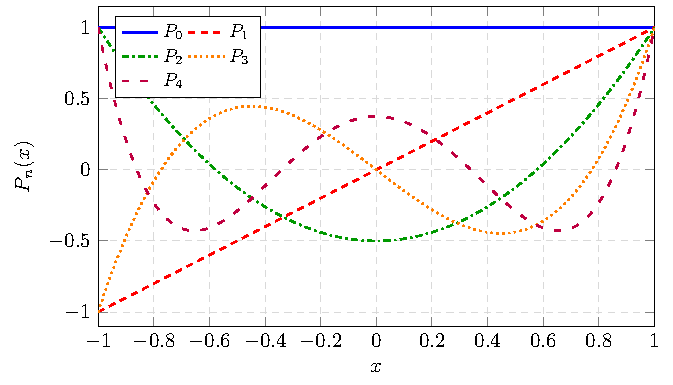
\includegraphics[width=0.86\linewidth]{figs/legendre-P.pdf}
\end{center}
Each $P_n$ is bounded on $[-1,1]$ and normalized by $P_n(1)=1$. Increasing $n$ adds
interior zeros while preserving $\int_{-1}^{1}P_m(x)P_n(x)\,dx=0$ for $m\ne n$
(proved in \eqref{eq:legendre-orthogonal-zero} on the orthogonality slide).
\end{frame}

\begin{frame}[allowframebreaks=1.00]{Rodrigues' formula}
\footnotesize

\textbf{What it is.} The recurrence \eqref{eq:legendre-recur} produces \(P_0,P_1,P_2,\dots\) one after another.
Rodrigues' formula gives any single \(P_n\) directly:
\begin{equation}
 P_n(x)=\frac{1}{2^n n!}\frac{d^n}{dx^n}(x^2-1)^n.
 \label{eq:rodrigues-legendre}
\end{equation}
\textbf{Why it is useful.} \((x^2-1)^n=(x-1)^n(x+1)^n\) has a zero of order \(n\) at each end \(x=\pm1\). So when we
integrate by parts, all boundary terms vanish. This makes the norm of \(P_n\) easy (next frame).

\textbf{Check \(n=2\) first:} \(\frac1{8}\frac{d^2}{dx^2}(x^4-2x^2+1)=\frac{12x^2-4}{8}=\frac{3x^2-1}{2}=P_2\). \checkmark

\textbf{Plan of the proof.} Show that the right side (1) has the same powers as \(P_n\), (2) has
coefficients obeying the same recurrence as \(P_n\), so it is a multiple of \(P_n\), and (3) equals \(1\) at
\(x=1\), so the multiple is \(1\).
\par\framebreak\par
\textbf{Step 1: expand and differentiate.} By the binomial theorem,
\[
 (x^2-1)^n=\sum_{k=0}^{n}\binom nk (x^2)^{n-k}(-1)^k=\sum_{k=0}^{n}(-1)^k\binom nk x^{2n-2k}.
\]
Differentiate \(n\) times. A power \(x^{2n-2k}\) survives only if \(2n-2k\ge n\), that is,
\(k\le n/2\), and then \(\frac{d^n}{dx^n}x^{2n-2k}=\frac{(2n-2k)!}{(n-2k)!}\,x^{n-2k}\). With
\(\binom nk\frac1{n!}=\frac{1}{k!\,(n-k)!}\),
\[
 \frac{1}{2^n n!}\frac{d^n}{dx^n}(x^2-1)^n
 =\sum_{k=0}^{\lfloor n/2\rfloor}
   c_k\,x^{n-2k},
 \qquad
 c_k=\frac{(-1)^k\,(2n-2k)!}{2^n\, k!\,(n-k)!\,(n-2k)!}.
\]
(\(\lfloor n/2\rfloor\) is the largest whole number \(\le n/2\).) So the powers are \(x^n,x^{n-2},x^{n-4},\dots\), the same
as in \(P_n\).
\par\framebreak\par
\textbf{Step 2: the ratio of neighbouring coefficients.} Divide \(c_{k+1}\) by \(c_k\). Most factorials cancel:
\((2n-2k-2)!/(2n-2k)!=1/[(2n-2k)(2n-2k-1)]\), \(k!/(k+1)!=1/(k+1)\),
\((n-k)!/(n-k-1)!=n-k\), \((n-2k)!/(n-2k-2)!=(n-2k)(n-2k-1)\). So
\[
 \frac{c_{k+1}}{c_k}
 =-\frac{(n-k)\,(n-2k)(n-2k-1)}{(k+1)\,(2n-2k)(2n-2k-1)}
 =-\frac{(n-2k)(n-2k-1)}{(2k+2)(2n-2k-1)},
\]
using \(\frac{n-k}{2n-2k}=\frac12\).

\textbf{Step 3: compare with the Legendre recurrence.} \eqref{eq:legendre-coeff-recurrence} links the coefficient \(a_j\)
of \(x^j\) to \(a_{j+2}\): \(\frac{a_j}{a_{j+2}}=-\frac{(j+2)(j+1)}{(n-j)(n+j+1)}\). Put \(j=n-2k-2\). Then \(a_{j+2}\) is the
coefficient of \(x^{n-2k}\) (that is, \(c_k\)) and \(a_j\) is that of \(x^{n-2k-2}\) (that is, \(c_{k+1}\)). Also
\[
 (j+2)(j+1)=(n-2k)(n-2k-1),\qquad n-j=2k+2,\qquad n+j+1=2n-2k-1,
\]
so \(a_j/a_{j+2}\) is exactly the ratio in Step~2. Same powers and same recurrence: the right side of
\eqref{eq:rodrigues-legendre} is a constant multiple of \(P_n\).
\par\framebreak\par
\textbf{Step 4: the constant is \(1\) (value at \(x=1\)).} Write \((x^2-1)^n=(x-1)^n(x+1)^n\) and use the Leibniz rule
\((fg)^{(n)}=\sum_{i=0}^{n}\binom ni f^{(i)}g^{(n-i)}\) with \(f=(x-1)^n\), \(g=(x+1)^n\). Every term with fewer than \(n\)
derivatives on \((x-1)^n\) still contains a factor \(x-1\), so it is \(0\) at \(x=1\). The only surviving term is
\(f^{(n)}g=n!\,(x+1)^n\), which at \(x=1\) equals \(n!\,2^n\). Dividing by \(2^nn!\) gives the value \(1\), so the
right side equals \(P_n\).

\smallskip
\textbf{Two consequences needed for the norm.}
The highest power in $(x^2-1)^n$ is $x^{2n}$. Hence
\[
 \frac{d^n}{dx^n}x^{2n}=\frac{(2n)!}{n!}x^n,
\]
and division by $2^n n!$ gives
\begin{equation}
 P_n(x)=\frac{(2n)!}{2^n(n!)^2}x^n+\text{lower powers}.
 \label{eq:legendre-leading}
\end{equation}
Differentiating \eqref{eq:legendre-leading} $n$ times removes all lower powers,
and $\frac{d^n}{dx^n}x^n=n!$ cancels one factor of $n!$:
\begin{equation}
 P_n^{(n)}(x)=\frac{(2n)!}{2^n n!}.
 \label{eq:legendre-nth-deriv}
\end{equation}
The zeros of order $n$ in $(x^2-1)^n$ at $x=\pm1$ also make the boundary terms
vanish when we integrate by parts up to $n$ times. These are the two facts the norm uses.

\textbf{Contour form (Schl\"afli).} Cauchy's derivative formula from Chapter~1,
$f^{(n)}(x)=\dfrac{n!}{2\pi i}\oint_C\dfrac{f(t)}{(t-x)^{n+1}}\,dt$, applied to
$f(t)=(t^2-1)^n$ in \eqref{eq:rodrigues-legendre} (the $n!$ cancels and
$2^n\cdot2\pi i=2^{n+1}\pi i$), also writes Rodrigues' formula as
\begin{equation}
 P_n(x)=\frac1{2^{n+1}\pi i}\oint_C\frac{(t^2-1)^n}{(t-x)^{n+1}}\,dt,
 \label{eq:schlafli-legendre}
\end{equation}
where $C$ is a simple counterclockwise contour enclosing $x$. The norm below uses the
derivative form; for Laguerre (later) the same Cauchy formula, read from contour to
derivative, gives Rodrigues' formula.
\end{frame}

\begin{frame}[allowframebreaks=1.00]{Orthogonality and norm of Legendre polynomials}
\footnotesize

Chapter~4's Legendre example already gave $\int_{-1}^1P_nP_m\,dx=0$ for $n\ne m$ from the
Sturm--Liouville theorem, but not $\int_{-1}^1P_n^2\,dx$; Rodrigues' formula gives both. The
goal is
\[
 \int_{-1}^{1}P_n(x)P_m(x)\,dx=\frac{2}{2n+1}\,\delta_{nm},
\]
which is \eqref{eq:legendre-orthogonality-full} below.

Assume without loss of generality that $m\ge n$. Use Rodrigues' formula \eqref{eq:rodrigues-legendre} for
the higher-degree polynomial:
\[
 \int_{-1}^{1}P_n(x)P_m(x)\,dx
 =\frac{1}{2^m m!}\int_{-1}^{1}
 P_n(x)\frac{d^m}{dx^m}(x^2-1)^m\,dx.
\]
Because $(x^2-1)^m=(x-1)^m(x+1)^m$ has a zero of order $m$ at each endpoint,
\[
 \left.\frac{d^j}{dx^j}(x^2-1)^m\right|_{x=\pm1}=0,
 \qquad 0\le j\le m-1.
\]
One integration by parts moves one derivative onto $P_n$ and costs a sign:
\[
 \int_{-1}^{1}P_n\,\frac{d^m}{dx^m}(x^2-1)^m\,dx
 =\Bigl[P_n\,\frac{d^{m-1}}{dx^{m-1}}(x^2-1)^m\Bigr]_{-1}^{1}
 -\int_{-1}^{1}P_n'\,\frac{d^{m-1}}{dx^{m-1}}(x^2-1)^m\,dx,
\]
and the bracket is zero because $\frac{d^{m-1}}{dx^{m-1}}(x^2-1)^m=0$ at $x=\pm1$ (case $j=m-1$). Repeating this $m$ times (all boundary
terms vanish, one sign per step) gives
\begin{equation}
 \int_{-1}^{1}P_nP_m\,dx
 =\frac{(-1)^m}{2^m m!}\int_{-1}^{1}
 P_n^{(m)}(x)(x^2-1)^m\,dx.
 \label{eq:legendre-rodrigues-ibp}
\end{equation}
If $m>n$, then $P_n^{(m)}=0$ because $P_n$ has degree $n$. Thus
\begin{equation}
  \int_{-1}^{1}P_n(x)P_m(x)\,dx=0
  \qquad(n\ne m).
  \label{eq:legendre-orthogonal-zero}
\end{equation}

For the diagonal case set $m=n$ in \eqref{eq:legendre-rodrigues-ibp}. Equation
\eqref{eq:legendre-nth-deriv} gives $P_n^{(n)}=(2n)!/(2^n n!)$, while
$(-1)^n(x^2-1)^n=(1-x^2)^n$. Therefore
\begin{equation}
 I_n:=\int_{-1}^{1}P_n(x)^2\,dx
 =\frac{(2n)!}{2^{2n}(n!)^2}\int_{-1}^{1}(1-x^2)^n\,dx.
 \label{eq:legendre-norm-ibp}
\end{equation}
To evaluate the remaining integral, set $x=2u-1$ (so $x=-1,1$ become $u=0,1$). Then $dx=2\,du$ and
$1-x^2=1-(4u^2-4u+1)=4u(1-u)$, so with the beta function of Chapter~2,
$B(p,q)=\int_0^1u^{p-1}(1-u)^{q-1}\,du=\Gamma(p)\Gamma(q)/\Gamma(p+q)$,
\begin{align*}
  \int_{-1}^{1}(1-x^2)^n\,dx
  &=2\cdot4^n\int_0^1u^n(1-u)^n\,du
  =2^{2n+1}B(n+1,n+1)\\
  &=2^{2n+1}\frac{\Gamma(n+1)^2}{\Gamma(2n+2)}
  =2^{2n+1}\frac{(n!)^2}{(2n+1)!}
  \qquad\bigl(\Gamma(k+1)=k!\bigr).
\end{align*}
Therefore
\[
  I_n
  =\frac{(2n)!}{2^{2n}(n!)^2}
    \cdot\frac{2^{2n+1}(n!)^2}{(2n+1)\,(2n)!}
  =\frac{2}{2n+1},
\]
using $(2n+1)!=(2n+1)\,(2n)!$; the factors $(2n)!$, $(n!)^2$, and $2^{2n}$ cancel.
Check: $n=0$ gives $\int_{-1}^1 1\,dx=2$.
Combining \eqref{eq:legendre-orthogonal-zero} ($n\ne m$) with this norm ($n=m$),
\begin{equation}
  \int_{-1}^{1}P_n(x)P_m(x)\,dx
  =\frac{2}{2n+1}\,\delta_{nm}.
  \label{eq:legendre-orthogonality-full}
\end{equation}
Why the value matters: $2/(2n+1)$ is exactly the denominator of every
Fourier--Legendre coefficient on the next slide.
\end{frame}

\begin{frame}[allowframebreaks=1.00]{Fourier--Legendre series}
\footnotesize

We want to expand a given $f$ on $[-1,1]$ in Legendre polynomials, as Chapter~4 expanded
in sines; that is, to find the coefficients $a_n$ in $f=\sum_n a_nP_n$. We quote \emph{completeness}: every $f$ with $\int_{-1}^1 f^2\,dx<\infty$ (the space
$L^2$ of Chapter~4) is the sum of such a series,
\[
  f(x)=\sum_{n=0}^{\infty}a_nP_n(x),
\]
in the mean-square sense $\int_{-1}^1\bigl(f-\sum_{n\le N}a_nP_n\bigr)^2dx\to0$.
Multiply by $P_m(x)$ and integrate term by term:
\begin{align*}
  \int_{-1}^{1}f(x)P_m(x)\,dx
  &=\sum_{n=0}^{\infty}a_n
    \int_{-1}^{1}P_n(x)P_m(x)\,dx
  =\sum_{n=0}^{\infty}a_n\frac{2}{2n+1}\,\delta_{nm}
  =a_m\frac{2}{2m+1},
\end{align*}
by the orthogonality relation \eqref{eq:legendre-orthogonality-full}.
Solving for $a_m$ gives
\begin{equation}
  a_m=\frac{2m+1}{2}\int_{-1}^{1}f(x)P_m(x)\,dx.
  \label{eq:fourier-legendre-coeff}
\end{equation}
Therefore the Fourier--Legendre expansion is
\begin{equation}
  f(x)=\sum_{n=0}^{\infty}
  \left[\frac{2n+1}{2}\int_{-1}^{1}f(s)P_n(s)\,ds\right]P_n(x).
  \label{eq:fourier-legendre}
\end{equation}

\emph{Example: $f(x)=|x|$.} Since $f$ is even and $P_n(-x)=(-1)^nP_n(x)$, $a_n=0$ for odd $n$. By \eqref{eq:fourier-legendre-coeff},
\[
  a_0=\frac12\int_{-1}^1|x|\,dx=\frac12,\qquad
  a_2=\frac52\cdot2\int_0^1x\,\frac{3x^2-1}{2}\,dx=\frac52\Bigl(\frac34-\frac12\Bigr)=\frac58,
\]
so, with $S_N=\sum_{n\le N}a_nP_n$, $|x|\approx S_2(x)=\frac12+\frac58P_2(x)=\frac{3+15x^2}{16}$.
By orthogonality, $\int_{-1}^1(f-S_N)^2dx=\int_{-1}^1f^2dx-\sum_{n\le N}a_n^2\frac{2}{2n+1}$, so each
added term can only lower the error:
\[
  \int_{-1}^1\bigl(|x|-S_N\bigr)^2dx=
  \begin{cases}\frac23-\frac12=\frac16,&N=0,\\[2pt] \frac23-\frac12-\frac{5}{32}=\frac1{96},&N=2.\end{cases}
\]
Adding $a_4=-3/16$ lowers the error to $1/384$. The corner at $x=0$ is matched slowest:
$S_2(0)=3/16$ instead of $0$.
\end{frame}

\begin{frame}{Useful formulas for the Legendre polynomial}
\footnotesize
\begin{center}
\renewcommand{\arraystretch}{1.55}
\begin{tabular}{ll}
differential equation
  & $(1-x^2)P_n'' - 2x\,P_n' + n(n+1)P_n = 0$ \\
series solution
  & $P_n(x)=\displaystyle\sum_{k=0}^{\lfloor n/2\rfloor}
       \frac{(-1)^k(2n-2k)!}{2^n k!\,(n-2k)!\,(n-k)!}\,x^{n-2k}$ \\
generating function
  & $\dfrac{1}{\sqrt{1-2xt+t^2}} = \displaystyle\sum_{n=0}^{\infty}P_n(x)\,t^n$ \\
recurrence
  & $(n+1)P_{n+1} = (2n+1)x\,P_n - n\,P_{n-1}$ \\
orthogonality
  & $\displaystyle\int_{-1}^{1}P_m(x)P_n(x)\,dx
       = \frac{2}{2n+1}\,\delta_{nm}$ \\
Rodrigues
  & $P_n(x)=\dfrac{1}{2^n n!}\dfrac{d^n}{dx^n}(x^2-1)^n$ \\
Schl\"afli
  & $P_n(x)=\dfrac{1}{2^{n+1}\pi i}
       \displaystyle\oint\frac{(t^2-1)^n}{(t-x)^{n+1}}\,dt$
       \quad \eqref{eq:schlafli-legendre}
\end{tabular}
\end{center}
\vspace{0.2em}
{\scriptsize The finite sum follows by expanding Rodrigues' formula;
$\lfloor n/2\rfloor$ means the greatest integer no larger than $n/2$.
Generating series: $|t|<1$ for $x\in[-1,1]$. The contour encloses $t=x$.}
\end{frame}

% ======================================================================
\section{Associated Legendre and spherical harmonics}
% ======================================================================

\begin{frame}[allowframebreaks=1.00]{Associated Legendre equation and $Y_n^m$}
\footnotesize

Most fields on a sphere also depend on the longitude $\phi$ (for example the potential of
charges placed off the polar axis), so we now drop axisymmetry.
Separate $y(\theta,\phi)=v(\theta)w(\phi)$. As in the two-dimensional polar case,
$2\pi$-periodicity lets us take $w=e^{im\phi}$ with $m\in\mathbb Z$.
Put $y=v(\theta)e^{im\phi}$ into the angular eigenproblem of \S\ref{sec:laplace-to-legendre},
\[
  \frac{1}{\sin\theta}
    \frac{\partial}{\partial\theta}
      \left(\sin\theta\,\frac{\partial y}{\partial\theta}\right)
  +\frac{1}{\sin^2\theta}\frac{\partial^2y}{\partial\phi^2}
  +\lambda y=0 .
\]
Since $\partial_\phi^2e^{im\phi}=-m^2e^{im\phi}$, every term carries the factor $e^{im\phi}\neq0$,
which cancels:
\[
  \frac{1}{\sin\theta}
    \frac{d}{d\theta}
      \left(\sin\theta\,\frac{dv}{d\theta}\right)
  +\left[\lambda-\frac{m^2}{\sin^2\theta}\right]v=0 .
\]
With $x=\cos\theta$, the first term becomes $\frac{d}{dx}\bigl[(1-x^2)v'\bigr]$ exactly as in
Step~1 of the axisymmetric frame, and $\sin^2\theta=1-x^2$. Hence
\begin{equation}
  \frac{d}{dx}\left[(1-x^2)v'(x)\right]
  +\left[
      \lambda-\frac{m^2}{1-x^2}
   \right]v(x)=0.
  \label{eq:assoc-legendre-general}
\end{equation}
As in Step~3 of the axisymmetric frame, finiteness at both poles fixes the eigenvalues (quoted):
$\lambda=n(n+1)$ with $n=|m|,|m|+1,\ldots$, and the equation becomes
\begin{equation}
 (1-x^2)v''-2xv'+\left[n(n+1)-\frac{m^2}{1-x^2}\right]v=0.
 \label{eq:assoc-legendre-expanded}
\end{equation}
Rather than a new series analysis, we build these solutions from the $P_n$ we already have.

\textbf{Derivative construction.} For $m=0,1,\ldots,n$ define
\begin{equation}
 P_n^m(x)=(-1)^m(1-x^2)^{m/2}\frac{d^mP_n(x)}{dx^m}.
 \label{eq:associated-legendre-definition}
\end{equation}
Picture: each $d/dx$ lowers the degree by one, and $(1-x^2)^{m/2}=\sin^m\theta$ vanishes at the
poles, as it must: there $\phi$ is undefined, so a mode carrying $e^{im\phi}$ ($m\ne0$) is
single-valued only if it is zero there. The sign $(-1)^m$ is a convention
(Condon--Shortley phase); some texts omit it.

\par\framebreak\par
\textbf{Why it solves \eqref{eq:assoc-legendre-expanded}: two steps.}

\emph{Step 1: differentiate the Legendre equation \(m\) times.} Start from
\((1-x^2)P_n''-2xP_n'+n(n+1)P_n=0\) and apply \(\frac{d^m}{dx^m}\) to each term, using the Leibniz rule
\((fg)^{(m)}=\sum_i\binom mi f^{(i)}g^{(m-i)}\). Since \(1-x^2\) has only two nonzero derivatives (\(-2x\) and \(-2\)), and
\(-2x\) only one (\(-2\)):
\begin{align*}
 \tfrac{d^m}{dx^m}\bigl[(1-x^2)P_n''\bigr]&=(1-x^2)P_n^{(m+2)}+m(-2x)P_n^{(m+1)}+\tbinom m2(-2)P_n^{(m)},\\
 \tfrac{d^m}{dx^m}\bigl[-2xP_n'\bigr]&=-2xP_n^{(m+1)}+m(-2)P_n^{(m)} .
\end{align*}
Write \(u=P_n^{(m)}\) and add, with \(n(n+1)u\). The \(u\) terms combine as
\(n(n+1)-m(m-1)-2m=n(n+1)-m(m+1)\):
\[
 (1-x^2)u''-2(m+1)xu'+\bigl[n(n+1)-m(m+1)\bigr]u=0 .
\]
\par\framebreak\par
\emph{Step 2: change the unknown.} Put \(u=(1-x^2)^{-m/2}v\), that is, \(v=(1-x^2)^{m/2}P_n^{(m)}\) (up to the sign
\((-1)^m\), this is \(P_n^m\)). By the product rule,
\[
 (1-x^2)^{m/2}u'=v'+\frac{mx\,v}{1-x^2},\qquad
 (1-x^2)^{m/2}u''=v''+\frac{2mx\,v'}{1-x^2}+\frac{m+m(m+1)x^2}{(1-x^2)^2}\,v .
\]
Multiply the equation of Step~1 by \((1-x^2)^{m/2}\) and insert these:
\begin{align*}
 &(1-x^2)v''+2mxv'+\frac{m+m(m+1)x^2}{1-x^2}v\\
 &\quad-2(m+1)xv'-\frac{2m(m+1)x^2}{1-x^2}v+\bigl[n(n+1)-m(m+1)\bigr]v=0 .
\end{align*}
\par\framebreak\par
\emph{Collect the terms.}
\begin{itemize}
  \item \(v'\): \(2mx-2(m+1)x=-2x\).
  \item \(v\): put everything over \(1-x^2\), writing \(m(m+1)=\frac{m(m+1)(1-x^2)}{1-x^2}\):
        \[
         \frac{m+m(m+1)x^2-2m(m+1)x^2-m(m+1)(1-x^2)}{1-x^2}+n(n+1).
        \]
        In the numerator the \(x^2\) terms cancel (\(m(m+1)-2m(m+1)+m(m+1)=0\)), leaving
        \(m-m(m+1)=-m^2\). So the \(v\) coefficient is \(n(n+1)-\frac{m^2}{1-x^2}\).
\end{itemize}
So \((1-x^2)v''-2xv'+\bigl[n(n+1)-\frac{m^2}{1-x^2}\bigr]v=0\), which is exactly \eqref{eq:assoc-legendre-expanded}.

For example, $P_1=x$ and $P_2=(3x^2-1)/2$ give
\[
 P_1^1=-\sqrt{1-x^2},\qquad
 P_2^1=-3x\sqrt{1-x^2},\qquad
 P_2^2=(1-x^2)\frac{d^2}{dx^2}\frac{3x^2-1}{2}=3(1-x^2).
\]
(Check $v=P_1^1$: $v'=x/\sqrt{1-x^2}$, $v''=(1-x^2)^{-3/2}$, and the left side of
\eqref{eq:assoc-legendre-expanded} reduces to $0$.)
For $m=0$ the construction returns $P_n$; for $m>n$ the derivative is zero, matching $n\ge|m|$.

\par\framebreak\par
\textbf{Spherical harmonics: name the angular modes.}
An unnormalized angular basis is
\[
  \mathcal Y_n^m(\theta,\phi)
    =P_n^{|m|}(\cos\theta)\,e^{im\phi},
  \qquad -n\le m\le n.
\]
The normalized spherical harmonics $Y_n^m$ differ from it by a constant and a fixed phase;
many texts write $\ell$ for the degree ($Y_{\ell m}$).
Combining the radial factors \eqref{eq:spherical-radial-powers} (keep $r^n$, regular at the origin)
with these angular factors, the regular interior expansion is
\begin{equation}
  \psi_{\mathrm{int}}(r,\theta,\phi)
    =\sum_{n=0}^{\infty}\sum_{m=-n}^{n}
      a_{nm}r^n\mathcal Y_n^m(\theta,\phi),
  \label{eq:laplace3d-sol}
\end{equation}
and the decaying exterior expansion uses $r^{-n-1}$ instead of $r^n$. There the $n=0,1,2$
terms are the monopole, dipole and quadrupole parts of the field.

(On a cone $\theta<\theta_0$ only $x=1$ must be regular, and non-integer degrees $\nu$ appear:
the Legendre functions $P_\nu$, quoted.)
\end{frame}

\begin{frame}[allowframebreaks=1.00]{Spherical-harmonic nodal patterns}
\footnotesize

\begin{center}
 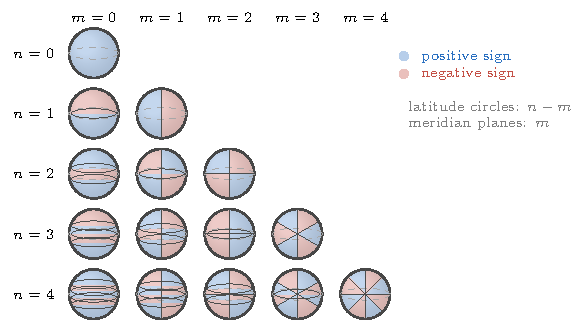
\includegraphics[width=0.74\linewidth]{figs/ch6_spherical_harmonics.pdf}
\end{center}
\scriptsize
Schematic counts, not exact nodal locations. Rows: degree $n$; columns: order $m$.
The factor $P_n^{|m|}(\cos\theta)$ has $n-|m|$ interior nodal latitudes. (By Rolle's theorem
applied to Rodrigues' formula, $P_n$ has $n$ zeros in $(-1,1)$; each derivative keeps one zero
between consecutive ones, so $d^{|m|}P_n/dx^{|m|}$, of degree $n-|m|$, has $n-|m|$ of them, and
$\sin^{|m|}\theta$ adds none inside.)
For $m>0$, a real factor $\cos(m\phi)$ or $\sin(m\phi)$ adds $m$ meridian planes;
for $m=0$, there are none.
\end{frame}

% ======================================================================
\section{Hermite polynomials}
% ======================================================================

\begin{frame}[allowframebreaks=1.00]{The Hermite equation and series solution}
\footnotesize

\textbf{Why this equation.} The quantum harmonic oscillator (two frames on) reduces to it,
and its polynomial solutions give the oscillator's states and energy levels.

\textbf{Step 1: substitute a power series.}  The physicists' Hermite polynomials solve
\begin{equation}
  y''-2xy'+2ny=0,
  \qquad n=0,1,2,\ldots.
  \label{eq:hermite-eq}
\end{equation}
Let $y(x)=\sum_{j=0}^{\infty}a_jx^j$.  Shifting indices as in the Legendre series (Step~2 of
\S\ref{sec:laplace-to-legendre}),
\[
  y''=\sum_{j=0}^{\infty}(j+2)(j+1)a_{j+2}x^j,
  \qquad
  -2xy'=-2x\sum_{j=1}^{\infty}ja_jx^{j-1}=-2\sum_{j=0}^{\infty}ja_jx^j .
\]
Substituting into \eqref{eq:hermite-eq} gives
$\sum_{j\ge0}\bigl[(j+2)(j+1)a_{j+2}+2(n-j)a_j\bigr]x^j=0$; every coefficient vanishes, so
\begin{equation}
  a_{j+2}=\frac{2(j-n)}{(j+2)(j+1)}a_j.
  \label{eq:hermite-coefficient-recurrence}
\end{equation}

\textbf{Step 2: termination condition.}  Even and odd chains are independent.  For integer
$n\ge0$, setting $j=n$ in \eqref{eq:hermite-coefficient-recurrence} gives
$a_{n+2}=\tfrac{2(n-n)}{(n+2)(n+1)}a_n=0$. Thus the same-parity chain terminates at degree $n$, giving a polynomial of exact degree
$n$.  The opposite-parity chain never hits a zero numerator, so we set its initial
coefficient to zero (the non-polynomial second solution of \eqref{eq:hermite-eq}).

\textbf{Step 3: explicit series from the downward product.}
Adopt the physicists' leading coefficient $a_n=2^n$ and run
\eqref{eq:hermite-coefficient-recurrence} \emph{downward} from degree $n$:
\[
  a_j=\frac{(j+2)(j+1)}{2(j-n)}\,a_{j+2},
\]
so $a_{n-2}=-\tfrac{n(n-1)}{4}\,a_n$ and $a_{n-4}=-\tfrac{(n-2)(n-3)}{8}\,a_{n-2}$. After $k$ steps, the numerator
contains the first $2k$ descending factors of $n!$, and the denominator is
$(-4)(-8)\cdots(-4k)=(-4)^k k!$. Hence
\[
 a_{n-2k}=\frac{n(n-1)\cdots(n-2k+1)}{(-4)^k k!}\,a_n
 =\frac{(-1)^k2^{n-2k}n!}{k!\,(n-2k)!},
\]
using $a_n=2^n$, $n(n-1)\cdots(n-2k+1)=n!/(n-2k)!$, and $2^n/(-4)^k=(-1)^k2^{n-2k}$.
Since $2^{n-2k}x^{n-2k}=(2x)^{n-2k}$, summing $a_{n-2k}x^{n-2k}$ over $k$ gives
\begin{equation}
  H_n(x)=\sum_{k=0}^{\lfloor n/2\rfloor}
  (-1)^k(2x)^{n-2k}\frac{n!}{k!(n-2k)!}.
  \label{eq:hermite-series}
\end{equation}
Low-$n$ checks: $H_0=1$, $H_1=2x$, $H_2=4x^2-2$, $H_3=8x^3-12x$.

Chapter~4's Hermite example puts \eqref{eq:hermite-eq} in Sturm--Liouville form
$(e^{-x^2}y')'+2ne^{-x^2}y=0$ ($p=w=e^{-x^2}$, eigenvalue $2n$) and gives
(the norm for $m=n$ comes from the generating function below)
\begin{equation}
  \int_{-\infty}^{\infty}H_n(x)H_m(x)e^{-x^2}\,dx=0\qquad(n\ne m).
  \label{eq:hermite-ortho}
\end{equation}
\end{frame}

\begin{frame}{Shapes of the first Hermite polynomials}
\footnotesize
\begin{center}
  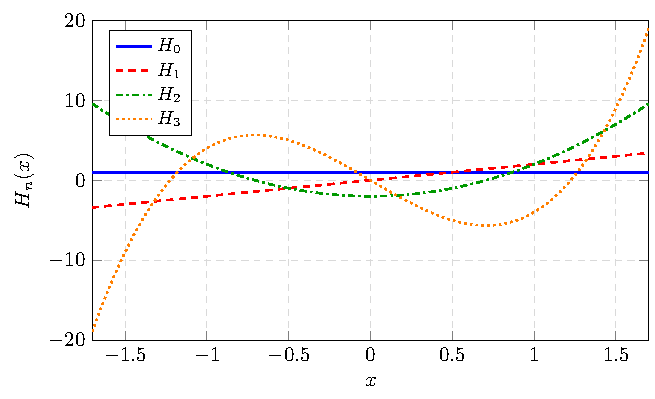
\includegraphics[width=0.86\linewidth]{figs/hermite-H.pdf}
\end{center}
Hermite polynomials grow away from the origin; the physical oscillator functions are
$e^{-\xi^2/2}H_n(\xi)$, with $\xi$ a scaled position (derived in the next frame).
\end{frame}

\begin{frame}[allowframebreaks=1.00]{Quantum harmonic oscillator}
\footnotesize

\textbf{Goal.} Find the allowed energies $E$ and the wavefunctions $\psi$ of a quantum particle in
a quadratic potential well. We will see that the Schr\"odinger equation reduces to Hermite's
equation, and that the requirement that $\psi$ be normalizable forces $E_n=(n+\tfrac12)\hbar\omega$.

Near the bottom of any potential well, $V$ is approximately quadratic, so the oscillator
models every small vibration (atoms in a molecule or a crystal).
For a mass-$M$ particle in $V(x)=\tfrac12 M\omega^2 x^2$ (angular frequency $\omega>0$), the
time-independent Schr\"odinger equation for the energy $E$ and spatial wavefunction $\psi$,
with $\hbar$ the reduced Planck constant, is
\[
  -\frac{\hbar^2}{2M}\psi''+\frac12 M\omega^2 x^2\psi=E\psi.
\]
Use $\xi=\sqrt{M\omega/\hbar}\,x$, so $d\xi/dx=\sqrt{M\omega/\hbar}$ and $x^2=\hbar\xi^2/(M\omega)$. Then
\[
 \frac{d^2\psi}{dx^2}=\frac{M\omega}{\hbar}\frac{d^2\psi}{d\xi^2},
 \qquad \frac12M\omega^2x^2=\frac12\hbar\omega\xi^2.
\]
Substitution gives
\[
 -\frac{\hbar^2}{2M}\frac{M\omega}{\hbar}\psi_{\xi\xi}+\frac12\hbar\omega\xi^2\psi
 =-\frac{\hbar\omega}{2}\psi_{\xi\xi}+\frac12\hbar\omega\xi^2\psi=E\psi;
\]
division by $\hbar\omega/2$ gives
$-\psi_{\xi\xi}+\xi^2\psi=(2E/\hbar\omega)\psi$, or
\begin{equation}
  \frac{d^2\psi}{d\xi^2}+\bigl(\varepsilon-\xi^2\bigr)\psi=0,
  \qquad
  \varepsilon=\frac{2E}{\hbar\omega}.
  \label{eq:qho-dimensionless}
\end{equation}


For large $|\xi|$, $\psi''-\xi^2\psi\approx0$ suggests the decaying factor
$e^{-\xi^2/2}$ (its second derivative is $(\xi^2-1)e^{-\xi^2/2}\approx\xi^2e^{-\xi^2/2}$, shown below).  Set
\[
  \psi(\xi)=e^{-\xi^2/2}\,y(\xi).
\]
Compute the derivatives by the product rule.  Write $f:=e^{-\xi^2/2}$, so
$f'=-\xi f$ and $f''=(-1+\xi^2)f$ (because
$f''=-(f+\xi f')=-(f+\xi(-\xi f))=(-1+\xi^2)f$).  Then
\begin{align*}
  \psi'
  &=f'y+fy'
  =e^{-\xi^2/2}\bigl(y'-\xi y\bigr),\\
  \psi''
  &=f''y+2f'y'+fy''\\
  &=e^{-\xi^2/2}\Bigl[
      (-1+\xi^2)y
      +2(-\xi)y'
      +y''
    \Bigr]\\
  &=e^{-\xi^2/2}\bigl(
      y''-2\xi y'+(\xi^2-1)y
    \bigr).
\end{align*}
Substitute into \eqref{eq:qho-dimensionless}:
\[
  \psi''+(\varepsilon-\xi^2)\psi
  =e^{-\xi^2/2}\Bigl[
      y''-2\xi y'+(\xi^2-1)y
      +(\varepsilon-\xi^2)y
    \Bigr]
  =e^{-\xi^2/2}\bigl[
      y''-2\xi y'+(\varepsilon-1)y
    \bigr].
\]
The Gaussian prefactor never vanishes, so
\begin{equation}
  y''-2\xi y'+(\varepsilon-1)y=0.
  \label{eq:qho-hermite-reduction}
\end{equation}
Equation \eqref{eq:qho-hermite-reduction} is \eqref{eq:hermite-eq} with $2n$ replaced by $\varepsilon-1$,
so the same series $y=\sum a_j\xi^j$ obeys \eqref{eq:hermite-coefficient-recurrence} with
$2(j-n)$ replaced by $2j-(\varepsilon-1)$:
\[
  a_{j+2}=\frac{2j+1-\varepsilon}{(j+2)(j+1)}a_j.
\]
\textbf{Why choose a terminating series?}
A bound state requires $\int_{-\infty}^{\infty}|\psi|^2\,d\xi<\infty$.
A polynomial $y$ times $e^{-\xi^2/2}$ satisfies this requirement.
In contrast, a nonterminating parity chain has
\[
 \frac{a_{j+2}}{a_j}\sim\frac{2}{j},
\]
like the coefficients of $e^{\xi^2}=\sum_k\xi^{2k}/k!$ (with $j=2k$, consecutive ones have ratio
$\tfrac{k!}{(k+1)!}=\tfrac{2}{j+2}$). Then $y$ grows like $e^{\xi^2}$ and $\psi$ like
$e^{\xi^2/2}$, which is not normalizable. So the chain must terminate, and the other parity
chain is set to zero.

\par\framebreak\par
Termination at degree $n$ means the numerator $2j+1-\varepsilon$ vanishes at $j=n$, i.e.
\[
  \varepsilon=2n+1,\qquad n=0,1,2,\ldots,
\]
and then $\varepsilon-1=2n$, so \eqref{eq:qho-hermite-reduction} is exactly the Hermite
equation \eqref{eq:hermite-eq}, $y''-2\xi y'+2ny=0$, with $\xi$ in place of $x$.  Since $\varepsilon=2E/(\hbar\omega)$, the energies are
therefore
\begin{equation}
  E_n=\Bigl(n+\frac12\Bigr)\hbar\omega,
  \qquad n=0,1,2,\ldots,
  \label{eq:energy-levels}
\end{equation}
and, since the polynomial solution of \eqref{eq:hermite-eq} is unique up to a constant (Step~2 of
the series frame), the spatial factors are
$\psi_n\propto e^{-\xi^2/2}H_n(\xi)$ with $H_n$ from \eqref{eq:hermite-series}.

\textbf{Physical reading.} The levels form an equally spaced ladder with step $\hbar\omega$,
and the lowest energy $\tfrac12\hbar\omega$ is not zero (zero-point energy): the particle cannot
sit at rest at the bottom of the well. The state $\psi_n$ has $n$ nodes (the zeros of $H_n$),
oscillates inside the classically allowed region $\xi^2<2n+1$ (where $\varepsilon>\xi^2$), and
decays like a Gaussian outside it.

\end{frame}

\begin{frame}[allowframebreaks=1.00]{Generating function, norm, and Rodrigues}
\footnotesize

\textbf{Step 1: generating function from the series.}  As for Legendre, a generating
function packs the whole family into one closed form, $g(x,t)=\sum_nH_n(x)t^n/n!$.
The coefficients of \eqref{eq:hermite-series} turn out to come from a product of two
exponentials:
\[
  g(x,t):=\exp(2xt-t^2)=e^{2xt}e^{-t^2}.
\]
Expand each exponential:
\[
  e^{2xt}=\sum_{m=0}^{\infty}\frac{(2x)^m}{m!}\,t^m,
  \qquad
  e^{-t^2}=\sum_{j=0}^{\infty}\frac{(-1)^j}{j!}\,t^{2j}.
\]
The product is a double sum.  The coefficient of $t^n$ arises from pairs $(m,j)$ with
$m+2j=n$, i.e.\ $m=n-2j$ for $j=0,\ldots,\lfloor n/2\rfloor$:
\begin{align*}
  [t^n]g(x,t)
  &=\sum_{j=0}^{\lfloor n/2\rfloor}
      \frac{(2x)^{n-2j}}{(n-2j)!}\cdot\frac{(-1)^j}{j!}\\
  &=\frac{1}{n!}
    \sum_{j=0}^{\lfloor n/2\rfloor}
      (-1)^j(2x)^{n-2j}\frac{n!}{j!\,(n-2j)!}.
\end{align*}
Comparing with the series solution \eqref{eq:hermite-series} (summation index $j$ in place of $k$),
the sum multiplying $1/n!$ is exactly $H_n(x)$, so $[t^n]g=H_n(x)/n!$.  Therefore
\begin{equation}
  g(x,t)=e^{-t^2+2xt}
  =\sum_{n=0}^{\infty}H_n(x)\frac{t^n}{n!}.
  \label{eq:hermite-gen}
\end{equation}

\textbf{Step 2: Rodrigues from $g=e^{x^2}e^{-(x-t)^2}$.}
Rewrite the exponent:
\[
  2xt-t^2=x^2-(x-t)^2,
  \qquad
  g(x,t)=e^{x^2}\,e^{-(x-t)^2}.
\]
We need the Taylor coefficients of $e^{-(x-t)^2}$ in $t$ at $t=0$. It depends on $x,t$ only
through $x-t$, so the chain rule gives
$\partial_t e^{-(x-t)^2}=2(x-t)e^{-(x-t)^2}=-\partial_x e^{-(x-t)^2}$; every derivative is again
a function of $x-t$, so $\partial/\partial t=-\partial/\partial x$ can be applied $n$ times:
\[
  \left.\frac{\partial^n}{\partial t^n}e^{-(x-t)^2}\right|_{t=0}
  =(-1)^n\frac{d^n}{dx^n}e^{-x^2}
  \quad\Longrightarrow\quad
  g(x,t)
  =\sum_{n=0}^{\infty}
    \Biggl[(-1)^ne^{x^2}\frac{d^n}{dx^n}e^{-x^2}\Biggr]
    \frac{t^n}{n!}.
\]
Matching coefficients with \eqref{eq:hermite-gen} gives Rodrigues' formula
\begin{equation}
  H_n(x)=(-1)^n e^{x^2}\frac{d^n}{dx^n}e^{-x^2}.
  \label{eq:hermite-rodrigues}
\end{equation}

\textbf{Step 3: recurrences from $\partial_t g$ and $\partial_x g$.}
Differentiate the closed form:
\[
  \frac{\partial g}{\partial t}=(2x-2t)g,
  \qquad
  \frac{\partial g}{\partial x}=2tg.
\]
Using the series \eqref{eq:hermite-gen},
\[
 \partial_tg=\sum_{n=1}^\infty H_n\frac{t^{n-1}}{(n-1)!}
            =\sum_{n=0}^\infty H_{n+1}\frac{t^n}{n!}.
\]
Multiplication by $t$ shifts the index in the other term:
\[
 2tg=\sum_{n=1}^\infty 2H_{n-1}\frac{t^n}{(n-1)!}
    =\sum_{n=1}^\infty 2nH_{n-1}\frac{t^n}{n!},
\]
where $1/(n-1)!=n/n!$. Thus the coefficient of $t^n/n!$ in $(2x-2t)g$ is
$2xH_n-2nH_{n-1}$. Comparing with $\partial_tg$ gives, for $n\ge1$,
\begin{equation}
  H_{n+1}(x)=2xH_n(x)-2nH_{n-1}(x).
  \label{eq:hermite-three-term}
\end{equation}
Likewise, $\partial_xg=2tg$ with the same power shift reads
$\sum_{n\ge0} H_n'\,t^n/n!=\sum_{n\ge1} 2nH_{n-1}\,t^n/n!$; comparing coefficients gives
\begin{equation}
 H_n'(x)=2nH_{n-1}(x),\qquad n\ge1.
 \label{eq:hermite-deriv-rec}
\end{equation}
\par\framebreak\par
\textbf{Step 4: norm via the double generating function.}
Idea: the product $g(x,s)g(x,t)$ contains every $H_mH_n$, as the coefficient of
$s^mt^n/(m!\,n!)$, so one Gaussian integral of the product computes the whole table of
integrals $\int H_mH_ne^{-x^2}dx$ at once. For real $s,t$ near $0$,
\begin{align*}
  I(s,t)
  &:=\int_{-\infty}^{\infty}e^{-x^2}g(x,s)g(x,t)\,dx
   =\int_{-\infty}^{\infty}
    e^{-x^2-s^2+2sx-t^2+2tx}\,dx.
\end{align*}
Complete the square in $x$:
\begin{align*}
  -x^2+2(s+t)x-s^2-t^2
  &=-\bigl[x-(s+t)\bigr]^2+(s+t)^2-s^2-t^2\\
  &=-\bigl[x-(s+t)\bigr]^2+2st,
\end{align*}
so, shifting $u=x-(s+t)$ and using $\int_{-\infty}^{\infty}e^{-u^2}\,du=\sqrt\pi$ from Chapter~2,
\[
  I(s,t)=e^{2st}\int_{-\infty}^{\infty}e^{-u^2}\,du
  =\sqrt\pi\,e^{2st}
  =\sqrt\pi\sum_{k=0}^{\infty}\frac{2^k}{k!}\,s^k t^k.
\]
On the other hand, expand both generating functions by \eqref{eq:hermite-gen} and integrate
term by term:
\[
  I(s,t)
  =\sum_{m,n=0}^{\infty}
    \Biggl(
      \int_{-\infty}^{\infty}H_m(x)H_n(x)e^{-x^2}\,dx
    \Biggr)
    \frac{s^m t^n}{m!\,n!}.
\]
Equate coefficients of $s^mt^n$. The closed form $\sqrt\pi\,e^{2st}$ has only diagonal powers
$s^kt^k$, so for $m\ne n$ the integral is $0$ (confirming \eqref{eq:hermite-ortho}); for $m=n$,
\[
  \frac{1}{(n!)^2}\int_{-\infty}^{\infty}H_n^2 e^{-x^2}\,dx=\sqrt\pi\,\frac{2^n}{n!}.
\]
Multiplying by $(n!)^2$ and combining both cases,
\begin{equation}
  \int_{-\infty}^{\infty}H_m(x)H_n(x)e^{-x^2}\,dx
  =2^n n!\sqrt\pi\,\delta_{mn}.
  \label{eq:hermite-norm}
\end{equation}
Low-$n$ check: $H_0=1$ and $\int_{-\infty}^{\infty}e^{-x^2}\,dx=\sqrt\pi$.
\end{frame}

\begin{frame}{Useful formulas for the Hermite polynomial}
\footnotesize
\begin{center}
\renewcommand{\arraystretch}{1.55}
\begin{tabular}{ll}
differential equation
  & $H_n'' - 2x\,H_n' + 2n\,H_n = 0$ \\
series solution
  & $H_n(x)=\displaystyle\sum_{k=0}^{\lfloor n/2\rfloor}
       (-1)^k(2x)^{n-2k}\,\frac{n!}{k!\,(n-2k)!}$ \\
generating function
  & $e^{-t^2+2tx} = \displaystyle\sum_{n=0}^{\infty}H_n(x)\,\frac{t^n}{n!}$ \\
recurrence
  & $H_n' = 2n\,H_{n-1}$,\quad
    $H_{n+1} = 2x\,H_n - 2n\,H_{n-1}$ \\
orthogonality
  & $\displaystyle\int_{-\infty}^{\infty}H_mH_n\,e^{-x^2}dx
       = n!\,2^n\sqrt{\pi}\,\delta_{mn}$ \\
Rodrigues
  & $H_n(x)=(-1)^ne^{x^2}\dfrac{d^n}{dx^n}e^{-x^2}$
\end{tabular}
\end{center}
Here $n\ge0$; the displayed recurrences use $n\ge1$, with $H_0=1$, $H_1=2x$.
\end{frame}

% ======================================================================
\section{Laguerre polynomials}
% ======================================================================

\begin{frame}[allowframebreaks=1.00]{Laguerre equation and its polynomial solutions}
\footnotesize

\textbf{Why this family.} We want polynomials that are orthogonal on the half-line
$[0,\infty)$. A radial coordinate $r$ lives there, and bound quantum states, such as
the electron in hydrogen, decay exponentially in $r$. The weight $e^{-x}$ builds
this decay in. Generalized Laguerre polynomials appear in the hydrogen radial
functions; here we study only the standard family, which solves
\begin{equation}
  x\,y''+(1-x)y'+n\,y=0,
  \qquad n=0,1,2,\ldots ,
  \label{eq:laguerre-eq}
\end{equation}
normalized by $L_n(0)=1$.

\textbf{Step 1: power series and coefficient recurrence.}
The point $x=0$ is regular singular (Chapter~3). Dividing by $x$ gives $P=(1-x)/x$ and $Q=n/x$,
so $p_0=\lim_{x\to0}xP=1$, $q_0=\lim_{x\to0}x^2Q=0$, and the indicial equation
$r(r-1)+p_0r+q_0=0$ becomes $r^2=0$. The root $r=0$ is repeated, so one solution is an
ordinary power series and the other contains $\ln x$ (Chapter~3). We keep the solution
that is finite at the origin.

Set $y=\sum_{k\ge0}a_k x^k$.  Then (shifting indices as for Legendre)
\[
  y'=\sum_{k\ge0}(k+1)a_{k+1}x^k,\qquad
  xy''=\sum_{k\ge0}k(k+1)a_{k+1}x^k,\qquad
  -xy'=-\sum_{k\ge0}k a_k x^k.
\]
Collecting the coefficient of $x^k$ in $xy''+y'-xy'+ny$ gives
\[
  k(k+1)a_{k+1}+(k+1)a_{k+1}+(n-k)a_k
  =(k+1)^2 a_{k+1}+(n-k)a_k.
\]
Setting every coefficient to zero yields the one-step recurrence
\begin{equation}
  a_{k+1}=-\frac{n-k}{(k+1)^2}\,a_k,\qquad k=0,1,2,\ldots.
  \label{eq:laguerre-coeff-recurrence}
\end{equation}
At $k=n$ one has $a_{n+1}=0$, so the series terminates as a polynomial of degree $n$.
With $a_0=1$ (so $L_n(0)=1$), iterating \eqref{eq:laguerre-coeff-recurrence} gives
\[
  a_k
  =\prod_{i=0}^{k-1}\Bigl(-\frac{n-i}{(i+1)^2}\Bigr)
  =(-1)^k\frac{n(n-1)\cdots(n-k+1)}{(k!)^2}
  =(-1)^k\frac{1}{k!}\binom{n}{k},
\]
using $n(n-1)\cdots(n-k+1)=k!\binom nk$, and therefore
\begin{equation}
  L_n(x)
   =\sum_{k=0}^{n}
      (-1)^k\binom{n}{k}\frac{x^k}{k!}.
  \label{eq:laguerre-series}
\end{equation}
The first few are $L_0=1$, $L_1=1-x$, $L_2=1-2x+\tfrac12 x^2$,
$L_3=1-3x+\tfrac32 x^2-\tfrac16 x^3$.
\end{frame}

\begin{frame}[allowframebreaks=1.00]{Laguerre orthogonality and norm}
\footnotesize

\textbf{Goal.} Show that $\int_0^\infty L_m(x)L_n(x)e^{-x}\,dx=\delta_{mn}$, that is, the
Laguerre polynomials are orthogonal on $[0,\infty)$ with weight $e^{-x}$, and already normalized.

\textbf{Step 2: Sturm--Liouville form and orthogonality.}
Multiplying \eqref{eq:laguerre-eq} by $e^{-x}$ and using
$\bigl(xe^{-x}y'\bigr)'=e^{-x}\bigl[xy''+(1-x)y'\bigr]$ produces the SL form
$\bigl(xe^{-x}y'\bigr)'+ne^{-x}y=0$ ($p=xe^{-x}$, $w=e^{-x}$, eigenvalue $n$).
As for Legendre and Hermite, the Chapter~4 boundary term
$xe^{-x}(L_nL_m'-L_n'L_m)$ vanishes at both ends: at $x=0$ because of the factor $x$,
and as $x\to\infty$ because $e^{-x}$ beats any polynomial. Hence, for $n\ne m$,
\begin{equation}
  \int_0^{\infty}L_n(x)L_m(x)e^{-x}\,dx=0.
  \label{eq:laguerre-ortho}
\end{equation}

\textbf{Step 3: generating function and the norm.}
To compute $\int_0^\infty L_n^2e^{-x}\,dx$ we use, as for Hermite, a generating function:
\begin{equation}
  g(x,t)
  :=\frac{1}{1-t}\exp\left(-\frac{xt}{1-t}\right)
  =\sum_{n=0}^{\infty}L_n(x)\,t^n,
  \qquad |t|<1.
  \label{eq:laguerre-gen}
\end{equation}
To check the second equality, expand the exponential and multiply each term
$\frac{1}{k!}\bigl(\frac{-xt}{1-t}\bigr)^k$ by $\frac1{1-t}$:
$g=\sum_{k\ge0}\frac{(-x)^k}{k!}\,\frac{t^{k}}{(1-t)^{k+1}}$.
Differentiating the geometric series $(1-t)^{-1}=\sum_{i\ge0}t^i$ $k$ times and dividing by $k!$ gives
$(1-t)^{-(k+1)}=\sum_{j\ge0}\binom{k+j}{k}t^j$.
So $t^{n}$ comes from $j=n-k$, $0\le k\le n$, with factor $\binom{n}{k}$, and
$[t^n]\,g=\sum_{k=0}^{n}\frac{(-x)^k}{k!}\binom{n}{k}=L_n(x)$ by \eqref{eq:laguerre-series}.

Now integrate two generating functions against the weight.
For real $s,t$ near zero, put
\[
 \alpha=1+\frac{s}{1-s}+\frac{t}{1-t}=\frac{1}{1-s}+\frac{t}{1-t}
 =\frac{(1-t)+t(1-s)}{(1-s)(1-t)}=\frac{1-st}{(1-s)(1-t)}>0.
\]
In the closed forms, the exponents of $e^{-x}$, $g(x,s)$, $g(x,t)$ add to $-\alpha x$, and
$\int_0^\infty e^{-\alpha x}\,dx=1/\alpha$. Integrating the series term by term on the left,
\begin{align*}
 \sum_{m,n\ge0}\Bigl(\int_0^{\infty}L_mL_ne^{-x}\,dx\Bigr)s^m t^n
 &=\int_0^\infty e^{-x}g(x,s)g(x,t)\,dx\\
 &=\frac1{(1-s)(1-t)\alpha}=\frac1{1-st}=\sum_{n=0}^{\infty}s^n t^n.
\end{align*}
Equating coefficients of $s^m t^n$ gives $0$ for $m\ne n$ (again \eqref{eq:laguerre-ortho}) and $1$ for $m=n$,
so the standard $L_n$ are already orthonormal (no normalizing constant is needed):
\begin{equation}
  \int_0^{\infty}L_m(x)L_n(x)e^{-x}\,dx=\delta_{mn}.
  \label{eq:laguerre-norm}
\end{equation}
\end{frame}

\begin{frame}[allowframebreaks=1.00]{Laguerre recurrences}
\footnotesize

\textbf{Goal.} Two recurrences for the Laguerre polynomials,
$(n+1)L_{n+1}=(2n+1-x)L_n-nL_{n-1}$ and $xL_n'=n(L_n-L_{n-1})$, both from the generating function
\eqref{eq:laguerre-gen}.

\textbf{Step 4: three-term recurrence from $\partial_t g$.}
A recurrence builds $L_{n+1}$ from $L_n$ and $L_{n-1}$ without the series.
From \eqref{eq:laguerre-gen}, the product and chain rules with
$\frac{d}{dt}\frac{1}{1-t}=\frac{d}{dt}\frac{t}{1-t}=\frac{1}{(1-t)^2}$ give
\[
  \frac{\partial g}{\partial t}
  =\frac{e^{-xt/(1-t)}}{(1-t)^2}-\frac{x\,e^{-xt/(1-t)}}{(1-t)^3}
  =g\cdot\frac{1-t-x}{(1-t)^2},
\]
or equivalently
\begin{equation}
  (1-t)^2\,\partial_t g=(1-t-x)\,g.
  \label{eq:laguerre-gen-dt}
\end{equation}
Expand both sides in powers of $t$, using $g=\sum_{n\ge0}L_n t^n$ and
$\partial_t g=\sum_{n\ge0}(n+1)L_{n+1}t^n$. On the left, multiplying by $t$ or $t^2$ shifts
the index down by one or two, so the pieces $1$, $-2t$, $t^2$ of $(1-t)^2$ contribute
$(n+1)L_{n+1}$, $-2nL_n$, $(n-1)L_{n-1}$ to $t^n$ (with $L_{-1}:=0$). On the right,
$(1-x)g$ gives $(1-x)L_n$ and $-tg$ gives $-L_{n-1}$. Equating,
\[
  (n+1)L_{n+1}-2nL_n+(n-1)L_{n-1}=(1-x)L_n-L_{n-1};
\]
moving $-2nL_n$ and $(n-1)L_{n-1}$ to the right, and using $(n-1)+1=n$, yields
\begin{equation}
  (n+1)L_{n+1}(x)
    =(2n+1-x)L_n(x)-nL_{n-1}(x).
  \label{eq:laguerre-three-term}
\end{equation}
Check at $n=1$: $2L_2=(3-x)L_1-L_0$ reads
$2-4x+x^2=(3-x)(1-x)-1$, which holds identically.

\textbf{Step 5: derivative recurrence.}
A second identity gives $L_n'$ without differentiating the series. Differentiating the
exponent of \eqref{eq:laguerre-gen} in $x$ gives $xg_x=-\frac{xt}{1-t}\,g$, while
\eqref{eq:laguerre-gen-dt} gives
\[
 t(1-t)g_t=tg\,\frac{1-t-x}{1-t}=tg-\frac{xt}{1-t}\,g=tg+xg_x .
\]
Thus $xg_x=tg_t-t^2g_t-tg$. Reading off $t^n$, where $tg_t\to nL_n$, $t^2g_t\to(n-1)L_{n-1}$,
$tg\to L_{n-1}$, gives, for $n\ge1$,
\begin{equation}
 xL_n'(x)=nL_n-(n-1)L_{n-1}-L_{n-1}=n\bigl[L_n(x)-L_{n-1}(x)\bigr].
 \label{eq:laguerre-derivative-recurrence}
\end{equation}
Check at $n=1$: $xL_1'=-x=1\cdot(L_1-L_0)$.
\end{frame}

\begin{frame}[allowframebreaks=1.00]{Laguerre Rodrigues formula from a contour integral}
\footnotesize

\textbf{Goal.} Derive Rodrigues' formula $L_n(x)=\frac{e^x}{n!}\frac{d^n}{dx^n}(x^ne^{-x})$,
which builds any single $L_n$ directly.

\textbf{Step 6: Schl{\"a}fli integral and Rodrigues formula.}
The $L_n$ are Taylor coefficients of $g$; Cauchy's formula writes them as contour
integrals, and a change of variable turns the integral into an $n$-th derivative, as for
Legendre in \eqref{eq:schlafli-legendre}. By Chapter~1, the coefficients of
$F(z)=\sum_{n\ge0}a_nz^n$ ($|z|<1$) are $a_n=\frac{1}{2\pi i}\oint_{|z|=\rho}F(z)\,z^{-n-1}\,dz$, $\rho<1$.
With $F(z)=g(x,z)$,
\begin{equation}
 L_n(x)=\frac{1}{2\pi i}\oint_{|z|=\rho}
 \frac{e^{-xz/(1-z)}}{(1-z)z^{n+1}}\,dz.
 \label{eq:laguerre-schlafli}
\end{equation}
For $x\ne0$, set $z=1-x/s$, i.e.\ $s=x/(1-z)$.  Then
\[
 1-z=\frac{x}{s},\qquad dz=\frac{x}{s^2}\,ds,\qquad
 -\frac{xz}{1-z}=x-s,\qquad z^{n+1}=\frac{(s-x)^{n+1}}{s^{n+1}},
\]
and the small circle around $z=0$ becomes a small counterclockwise loop around $s=x$
(since $s\approx x(1+z)$ for small $z$). Substituting into \eqref{eq:laguerre-schlafli},
\[
 L_n(x)=\frac{1}{2\pi i}\oint
 e^{x-s}\cdot\frac{s}{x}\cdot\frac{s^{n+1}}{(s-x)^{n+1}}\cdot\frac{x}{s^2}\,ds
 =\frac{e^x}{2\pi i}\oint
 \frac{s^ne^{-s}}{(s-x)^{n+1}}\,ds.
\]
Cauchy's derivative formula from Chapter~1,
$\frac{1}{2\pi i}\oint\frac{f(s)}{(s-x)^{n+1}}\,ds=\frac{f^{(n)}(x)}{n!}$ with $f(s)=s^ne^{-s}$,
now yields Rodrigues' formula (at $x=0$ by continuity):
\begin{equation}
 L_n(x)=\frac{e^x}{n!}\frac{d^n}{dx^n}\bigl(x^ne^{-x}\bigr).
 \label{eq:laguerre-rodrigues}
\end{equation}
\textbf{Example ($n=2$).} Two product-rule steps give
$\frac{d}{dx}(x^2e^{-x})=(2x-x^2)e^{-x}$ and
$\frac{d^2}{dx^2}(x^2e^{-x})=(2-4x+x^2)e^{-x}$, so
$L_2=\frac12(2-4x+x^2)=1-2x+\frac12x^2$, matching \eqref{eq:laguerre-series}.
\end{frame}

\begin{frame}{Shapes of the first Laguerre polynomials}
\footnotesize
\begin{center}
  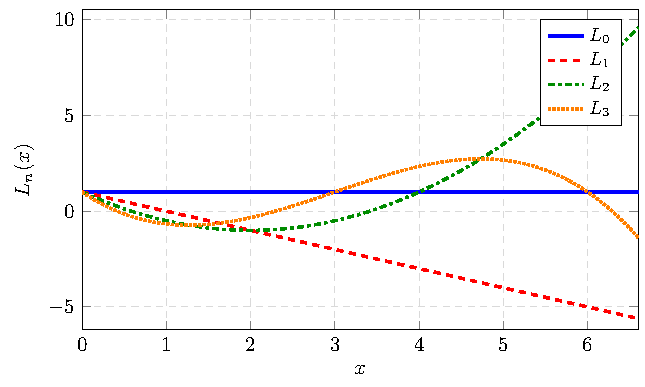
\includegraphics[width=0.86\linewidth]{figs/laguerre-L.pdf}
\end{center}
All standard Laguerre polynomials satisfy $L_n(0)=1$. The weight $e^{-x}$ makes them
natural on $[0,\infty)$.
\end{frame}

\begin{frame}{Useful formulas for the Laguerre polynomial}
\footnotesize
\begin{center}
\renewcommand{\arraystretch}{1.55}
\begin{tabular}{ll}
differential equation
  & $xL_n''+(1-x)L_n'+nL_n=0$ \\
series / first polynomials
  & $L_n(x)=\displaystyle\sum_{k=0}^{n}
       (-1)^k\binom{n}{k}\dfrac{x^k}{k!}$ \\
  & $L_0=1,\; L_1=1-x,\; L_2=1-2x+\tfrac12 x^2$ \\
generating function
  & $\dfrac{1}{1-t}\exp\left(-\dfrac{xt}{1-t}\right)
       =\displaystyle\sum_{n=0}^{\infty}L_n(x)t^n$ \\
recurrence
  & $(n+1)L_{n+1}=(2n+1-x)L_n-nL_{n-1}$ \\
  & $xL_n'=n(L_n-L_{n-1})$ \\
orthonormality
  & $\displaystyle\int_0^{\infty}L_mL_n\,e^{-x}\,dx=\delta_{mn}$ \\
Rodrigues
  & $L_n=\dfrac{e^x}{n!}\dfrac{d^n}{dx^n}(x^ne^{-x})$
\end{tabular}
\end{center}
{\scriptsize Generating series requires $|t|<1$.}
\end{frame}

% ======================================================================
\section{Chebyshev polynomials}
% ======================================================================

\begin{frame}[allowframebreaks=1.00]{Definition through $\cos n\theta$}
\footnotesize

We want polynomials that behave like $\cos n\theta$: then a cosine series becomes a
polynomial expansion on $[-1,1]$ that inherits the simple zeros and orthogonality of cosines.
The Chebyshev polynomial of the first kind is defined by
\begin{equation}
  T_n(\cos\theta)=\cos(n\theta).
  \label{eq:cheby-def}
\end{equation}
That is, set $x=\cos\theta$ and read off a polynomial in $x$:
\[
  T_0(x)=1,\qquad
  T_1(x)=x,\qquad
  T_2(x)=2x^2-1,\qquad
  T_3(x)=4x^3-3x.
\]
(For $T_2$: $\cos2\theta=2\cos^2\theta-1$.  For $T_3$: $\cos3\theta=4\cos^3\theta-3\cos\theta$.)

\textbf{Recurrence from angle addition.}  Adding
$\cos((n+1)\theta)=\cos(n\theta)\cos\theta-\sin(n\theta)\sin\theta$ and
$\cos((n-1)\theta)=\cos(n\theta)\cos\theta+\sin(n\theta)\sin\theta$ cancels the sines, $T_{n+1}(x)+T_{n-1}(x)=2xT_n(x)$, so
\begin{equation}
  T_{n+1}(x)=2xT_n(x)-T_{n-1}(x),
  \qquad n\ge1,
  \label{eq:cheby-recur}
\end{equation}
with $T_0=1$, $T_1=x$. The leading term of $2xT_n$ cannot cancel with $T_{n-1}$, so
the degree rises by one and the leading coefficient doubles at each step: $T_n$ has
leading coefficient $2^{n-1}$ for $n\ge1$.

Setting $\theta=0,\pi$ gives $T_n(1)=1$ and $T_n(-1)=(-1)^n$.  Replacing $\theta$ by
$\pi-\theta$ sends $x\to-x$ and $\cos n\theta\to\cos(n\pi-n\theta)=(-1)^n\cos n\theta$ (as $\sin n\pi=0$), so
$T_n(-x)=(-1)^nT_n(x)$.

\textbf{Generating function.}  For real $|t|<1$ and $x=\cos\theta\in[-1,1]$,
$T_n(x)t^n=\operatorname{Re}(te^{i\theta})^n$.  Sum the geometric series and multiply above and below by
$1-te^{-i\theta}$, using $(1-te^{i\theta})(1-te^{-i\theta})=1-2t\cos\theta+t^2$:
\begin{equation}
  \sum_{n=0}^{\infty}T_n(x)\,t^{n}
  =\operatorname{Re}\frac{1}{1-te^{i\theta}}
  =\operatorname{Re}\frac{1-te^{-i\theta}}{1-2t\cos\theta+t^{2}}
  =\frac{1-xt}{1-2xt+t^{2}}.
  \label{eq:cheby-gen}
\end{equation}

\textbf{Differential equation via the chain rule.}
Set $x=\cos\theta$ and $Y(\theta):=T_n(\cos\theta)=\cos(n\theta)$, so
$Y''(\theta)=-n^2 Y(\theta)$.  The chain rule with $dx/d\theta=-\sin\theta$ gives
$dY/d\theta=-\sin\theta\,T_n'(x)$; differentiating once more (product rule),
\[
  \frac{d^2Y}{d\theta^2}
  =-\cos\theta\,T_n'(x)-\sin\theta\bigl(-\sin\theta\,T_n''(x)\bigr)
  =-\cos\theta\,T_n'(x)+\sin^2\theta\,T_n''(x).
\]
Substitute $\cos\theta=x$, $\sin^2\theta=1-x^2$ and $Y''=-n^2T_n$; this is the Chebyshev equation
\begin{equation}
  (1-x^2)T_n''(x)-xT_n'(x)+n^2T_n(x)=0.
  \label{eq:cheby-eq}
\end{equation}
\end{frame}

\begin{frame}{Shapes of the first Chebyshev polynomials}
\footnotesize
\begin{center}
  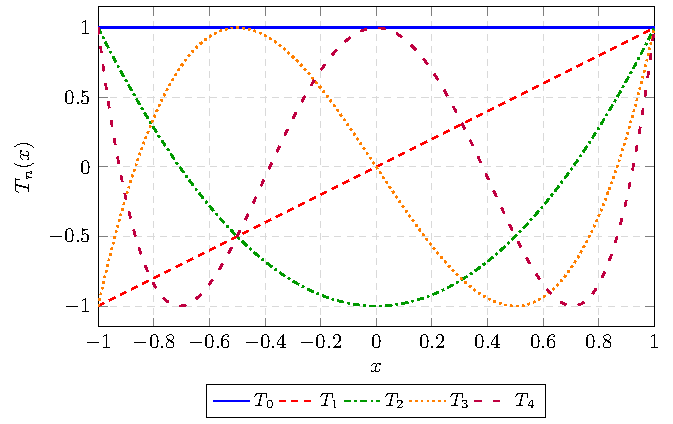
\includegraphics[width=0.86\linewidth]{figs/chebyshev-T.pdf}
\end{center}
$T_n(\cos\theta)=\cos(n\theta)$ keeps every $T_n$ between $-1$ and $1$ on $[-1,1]$.
\end{frame}

\begin{frame}[allowframebreaks=1.00]{Chebyshev nodes and orthogonality}
\footnotesize

\textbf{Zeros (nodes).} For $n\ge1$ and $x=\cos\theta\in[-1,1]$ with $\theta\in[0,\pi]$, the definition \eqref{eq:cheby-def} gives
\[
  T_n(x)=0\iff\cos(n\theta)=0
  \iff\theta_k=\frac{(2k-1)\pi}{2n},
  \quad k=1,\ldots,n.
\]
\begin{equation}
  x_k=\cos\left(\frac{(2k-1)\pi}{2n}\right),
  \qquad k=1,\ldots,n.
  \label{eq:cheby-nodes}
\end{equation}
The angles are equally spaced, but $x=\cos\theta$ crowds the nodes near $\pm1$.
This is what interpolation needs: the error of the polynomial through $n$ nodes contains
the factor $\prod_k(x-x_k)$ (quoted), which for these nodes equals $T_n(x)/2^{n-1}$ (same zeros and
leading coefficient), so it never exceeds $2^{1-n}$ and ripples evenly.  For equally spaced
nodes this factor is largest near $\pm1$, where the interpolant can blow up (Runge's phenomenon, e.g.\ for $1/(1+25x^2)$).
\begin{center}
  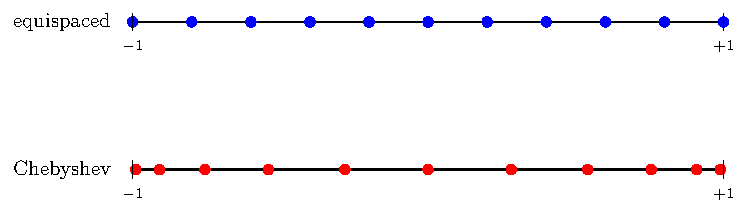
\includegraphics[width=0.72\linewidth]{figs/chebyshev-nodes.pdf}
\end{center}

\textbf{Orthogonality.}
We want the weight that turns $\int T_nT_m\,w\,dx$ into cosine orthogonality.  Since
$dx=-\sin\theta\,d\theta=-\sqrt{1-x^2}\,d\theta$, the choice is $w=1/\sqrt{1-x^2}$.
It is also the Sturm--Liouville weight: as
$(\sqrt{1-x^2}\,T_n')'=[(1-x^2)T_n''-xT_n']/\sqrt{1-x^2}$, dividing \eqref{eq:cheby-eq} by
$\sqrt{1-x^2}$ gives the Chapter~4 form with $p=\sqrt{1-x^2}$, $w=1/\sqrt{1-x^2}$, $\lambda=n^2$.

Substitute $x=\cos\theta$: as $x$ runs from $-1$ to $1$, $\theta$ runs from $\pi$ down to $0$,
and $\sqrt{1-x^2}=\sin\theta$ for $\theta\in[0,\pi]$.  Therefore
\begin{align*}
  \int_{-1}^{1}
    \frac{T_n(x)T_m(x)}{\sqrt{1-x^2}}\,dx
  &=\int_{\pi}^{0}
      \frac{T_n(\cos\theta)\,T_m(\cos\theta)}{\sin\theta}
      (-\sin\theta)\,d\theta
  =\int_0^{\pi}\cos(n\theta)\cos(m\theta)\,d\theta,
\end{align*}
by \eqref{eq:cheby-def}.  For $n\ne m$, use $\cos A\cos B=[\cos(A-B)+\cos(A+B)]/2$:
\[
 \int_0^\pi\cos(n\theta)\cos(m\theta)\,d\theta
 =\frac12\left[\frac{\sin((n-m)\theta)}{n-m}
              +\frac{\sin((n+m)\theta)}{n+m}\right]_0^\pi=0.
\]
For $n=m\ge1$, use $\cos^2(n\theta)=[1+\cos(2n\theta)]/2$:
\[
 \int_0^\pi\cos^2(n\theta)\,d\theta
 =\left[\frac\theta2+\frac{\sin(2n\theta)}{4n}\right]_0^\pi=\frac\pi2.
\]
For $n=m=0$, the integrand is $1$ and the integral is $\pi$.
Hence
\begin{equation}
  \int_{-1}^{1}
    \frac{T_n(x)T_m(x)}{\sqrt{1-x^2}}\,dx
  =
  \begin{cases}
    \pi, & n=m=0,\\[0.2em]
    \pi/2, & n=m\ge1,\\[0.2em]
    0, & n\ne m.
  \end{cases}
  \label{eq:cheby-ortho}
\end{equation}
\end{frame}

\begin{frame}{Useful formulas for the Chebyshev polynomial}
\footnotesize
\begin{center}
\renewcommand{\arraystretch}{1.55}
\begin{tabular}{ll}
definition
  & $T_n(\cos\theta)=\cos(n\theta)$ \\
differential equation
  & $(1-x^2)T_n''-xT_n'+n^2T_n=0$ \\
first polynomials
  & $T_0=1,\; T_1=x,\; T_2=2x^2-1,\; T_3=4x^3-3x$ \\
recurrence
  & $T_{n+1}=2xT_n-T_{n-1}$ \\
generating function
  & $\dfrac{1-xt}{1-2xt+t^2}
       =\displaystyle\sum_{n=0}^{\infty}T_n(x)t^n$, \;\eqref{eq:cheby-gen} \\
zeros
  & $x_k=\cos\left(\dfrac{(2k-1)\pi}{2n}\right)$ \\
orthogonality
  & $\displaystyle\int_{-1}^{1}
       \dfrac{T_nT_m}{\sqrt{1-x^2}}\,dx
       =\begin{cases}
          \pi, & n=m=0,\\
          \pi/2, & n=m\ge1,\\
          0, & n\ne m .
        \end{cases}$
\end{tabular}
\end{center}
{\scriptsize Generating series requires $|t|<1$.}
\end{frame}

% ======================================================================
\section{Summary}
% ======================================================================

\begin{frame}{Summary: four orthogonal families}
\footnotesize
\begin{center}
\renewcommand{\arraystretch}{1.45}
\begin{tabular}{llll}
\textbf{Family} & \textbf{Interval} & \textbf{Weight} & \textbf{ODE (sketch)} \\
\hline
Legendre $P_n$
  & $[-1,1]$
  & $1$
  & $(1-x^2)y''-2xy'+n(n+1)y=0$ \\
Hermite $H_n$
  & $(-\infty,\infty)$
  & $e^{-x^2}$
  & $y''-2xy'+2ny=0$ \\
Laguerre $L_n$
  & $[0,\infty)$
  & $e^{-x}$
  & $xy''+(1-x)y'+ny=0$ \\
Chebyshev $T_n$
  & $[-1,1]$
  & $(1-x^2)^{-1/2}$
  & $(1-x^2)y''-xy'+n^2y=0$ \\
\end{tabular}
\end{center}
\vspace{0.5em}
{\footnotesize
\textbf{Physical origins (one line each).}
 $P_n$: axisymmetric Laplace / multipoles;
$H_n$: quantum harmonic oscillator;
$L_n$: its generalized family occurs in the hydrogen radial equation;
$T_n$: $\cos n\theta$ and stable interpolation.
}

\vspace{0.4em}
Each family has a Sturm--Liouville ODE, a recurrence, and orthogonality on its own interval
and weight, so each supports series expansions just as Fourier series use $e^{inx}$.
\end{frame}

\begin{frame}[allowframebreaks=1.00]{Why the expansions converge: completeness}
\footnotesize

Orthogonality finds the coefficients; completeness says the series really reproduces $f$.
For any of the four families, with polynomials $\phi_n$, interval $I$ and weight $w$ from the table,
\[
 c_n=\frac{\displaystyle\int_I f(x)\phi_n(x)w(x)\,dx}
            {\displaystyle\int_I\phi_n(x)^2w(x)\,dx},
 \qquad S_N(x)=\sum_{n=0}^N c_n\phi_n(x).
\]
Completeness (quoted, as for $P_n$ on the Fourier--Legendre slide) states
\[
 \int_I|f(x)-S_N(x)|^2w(x)\,dx\longrightarrow0
 \quad\text{whenever}\quad\int_I|f(x)|^2w(x)\,dx<\infty.
\]
This is \emph{mean-square} convergence: the weighted area of the squared error tends to
zero, not the error at every point.  For example, the Legendre sums of the step
$\operatorname{sgn}x$ overshoot to about $1.18$ next to the jump for every large $N$, yet their
squared-error area shrinks to zero because the overshoot region narrows.

\medskip
\textbf{The common workflow.} Choose the family from the differential equation
and its interval; identify the weight; compute coefficients by orthogonality;
use a finite sum as an approximation.
\end{frame}

\end{document}
